\documentclass[10pt]{article}
\usepackage[utf8]{inputenc}

\renewcommand{\figurename}{\textbf{Appendix Figure}}
\renewcommand{\thefigure}{\textbf{S\arabic{figure}}}

\usepackage{caption}
\captionsetup[figure]{font=small}

\usepackage{amsmath}
\usepackage{amsthm}
\usepackage{amssymb}
\usepackage{bbm}
\usepackage{mathrsfs}
\usepackage{mathtools}
\usepackage{hyperref}
\usepackage{xcolor}
%%%%%%%%%%%%%%%%%%%%%%%%%%%%%%%%%%%%%%%%%
\setlength{\tabcolsep}{20pt}
\textwidth16cm
\oddsidemargin0.4cm
\renewcommand{\baselinestretch}{1.3} 	% Einstellung Zeilenabstand
\renewcommand{\jot}{8pt}
%%%%%%%%%%%%%%%%%%%%%%%%%%%%%%%%%%%%%%%%%
% Vectors (greek)
\newcommand{\bfalpha}{\boldsymbol{\alpha}}
\newcommand{\bfbeta}{\boldsymbol{\beta}}
\newcommand{\bfpsi}{\boldsymbol{\psi}}
\newcommand{\bftheta}{\boldsymbol{\theta}}
% Vectors
\newcommand{\bfx}{\mathbf{x}}
\newcommand{\bfy}{\mathbf{y}}
\newcommand{\bfa}{\mathbf{a}}
\newcommand{\bfb}{\mathbf{b}}
\newcommand{\bfc}{\mathbf{c}}
\newcommand{\bfg}{\mathbf{g}}
\newcommand{\bfm}{\mathbf{m}}
\newcommand{\bfu}{\mathbf{u}}
\newcommand{\bfz}{\mathbf{z}}
%%%%%%%%%%%%%%%%%%%%%%%%%%%%%%%%%%%%%%%%%
\newtheorem{env_def}{Definition}
\newtheorem{env_thm}{Theorem}
\newtheorem{env_lem}{Lemma}
\newtheorem{env_prop}{Proposition}
\newtheorem{env_exm}{Example}
\newtheorem{env_cor}{Corollary}
\newtheorem{env_obs}{Observation}
%%%%%%%%%%%%%%%%%%%%%%%%%%%%%%%%%%%%%%%%%
\DeclareMathOperator*{\diag}{diag}
\DeclareMathOperator*{\eigenv}{eigenvalues}
\DeclareMathOperator*{\var}{Var}
\DeclareMathOperator*{\expect}{\mathbb{E}}
\DeclareMathOperator*{\tr}{tr}
\DeclareMathOperator*{\kl}{KL}
\DeclareMathOperator*{\argmin}{arg\min}
\DeclareMathOperator*{\argmax}{arg\max}
\DeclareMathOperator*{\BETA}{Beta}
\DeclareMathOperator*{\BINOM}{Bin}
\DeclareMathOperator*{\BETABINOM}{Beta-Binomial}
\DeclareMathOperator*{\BERNOULLI}{Bernoulli}
\DeclareMathOperator*{\NORMAL}{\mathcal{N}}
\DeclareMathOperator*{\LOGNORMAL}{LogNormal}
\DeclareMathOperator*{\IWISHART}{\mathcal{W}^{-1}}
\DeclareMathOperator*{\IGAMMA}{IG}
%%%%%%%%%%%%%%%%%%%%%%%%%%%%%%%%%%%%%%%%%
\newcommand{\sprod}[2]{\langle #1, #2 \rangle}
%%%%%%%%%%%%%%%%%%%%%%%%%%%%%%%%%%%%%%%%%
\title{Appendix for: \\

\vspace{2ex}

\veryverylarge\textbf{CellRegMap: A statistical framework for mapping  context-specific regulatory variants using single cell RNA-sequencing.} 
\vspace{1ex}
% \\ \verylarge\textbf{Supplementary Methods}
}
\author{Anna S.E. Cuomo, Tobias Heinen, Danai Vagiaki, Danilo Horta, \\
John C. Marioni, Oliver Stegle }
% \author{Cuomo A.S.E., Heinen T., Vagiaki D., Horta D., Marioni J.C., Stegle O.}
\date{}
% \title{\verylarge\textbf{Supplementary Methods}}
% \author{}
% \date{}

\setlength\parindent{0pt}

\begin{document}

\maketitle
% \pagebreak
% \clearpage
% \cleardoublepage

\tableofcontents

\section{Supplementary Figures}\label{sec:SupplementaryFigures} 


\begin{figure}[h]
    \centering
    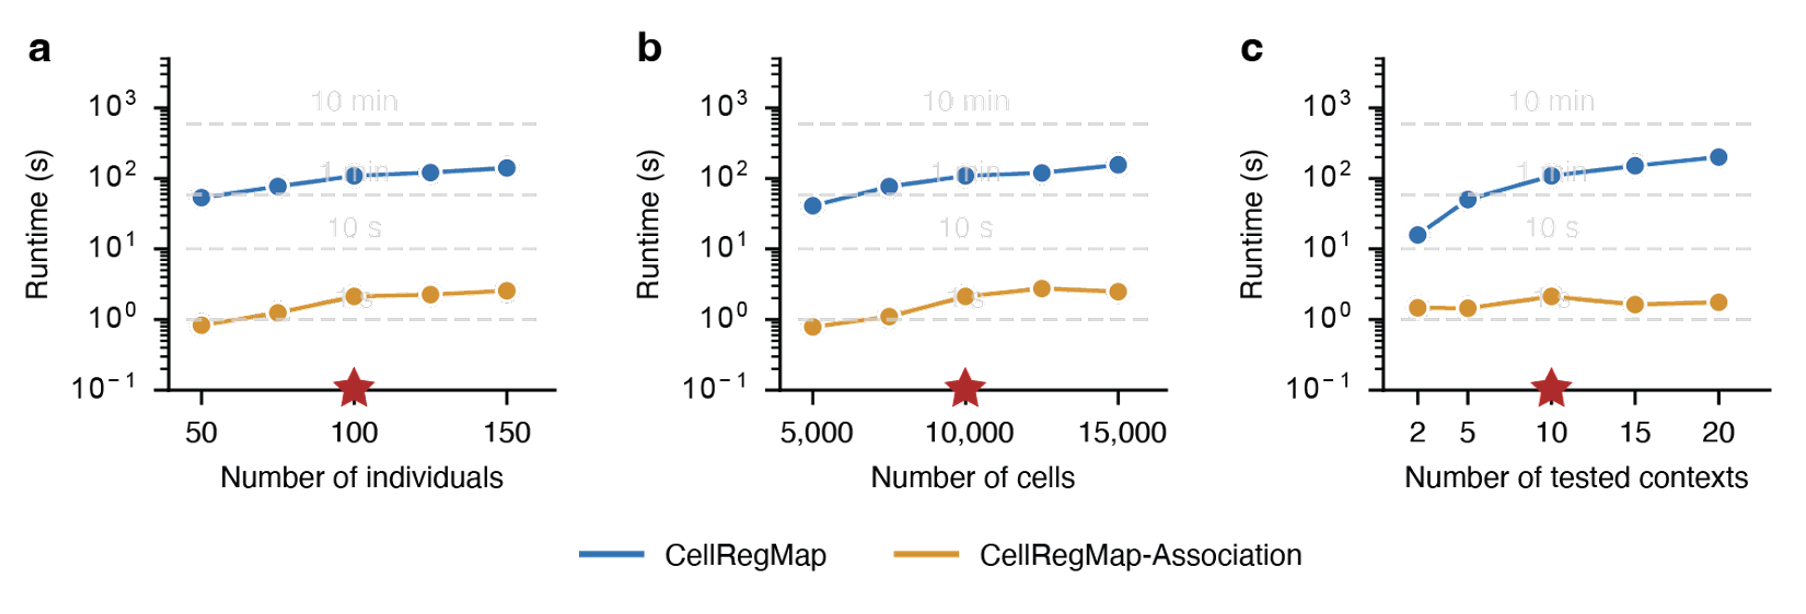
\includegraphics[width=16cm]{Appendix_CellRegMap/SuppFigures/Fig_S1.png}
    \caption{\textbf{Empirical assessment of the computational complexity of CellRegMap and CellRegMap-Association test.} 
    Shown are empirical runtimes for simulated data (setup as described in \textbf{Materials and Methods}) averaged across 150 eQTL. 
    Runtimes evaluated on an Intel Xeon CPU E5-2660 v4 with 2.00GHz. 
    Shown are runtimes (y-axis) for testing a single eQTL as a function of the number of individuals \textbf{(a)}, the total number of cells \textbf{(b)} and the number of context variables \textbf{(c)}; runtimes are evaluated for both the CellRegMap model (interaction test, blue), and the corresponding association test (orange). 
    Stars highlight default values for fixed parameters. 
    All parameters retained at their default parameter values except the parameter that is indicated on the x axis.}
\end{figure}

\begin{figure}[htb!]
    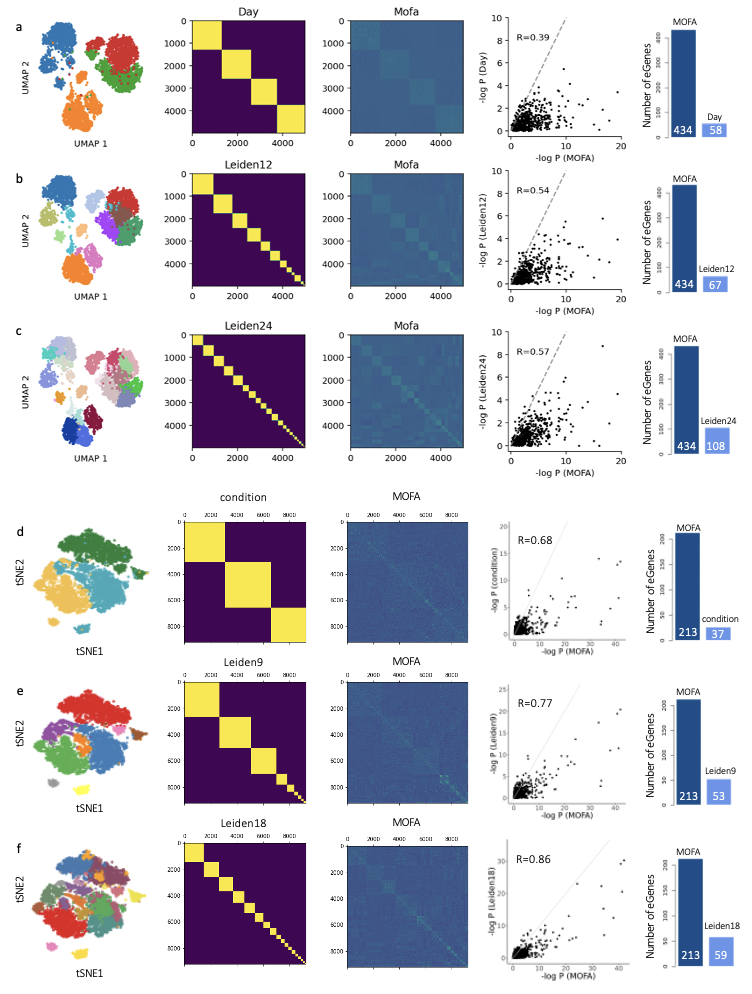
\includegraphics[width=15cm]{Appendix_CellRegMap/SuppFigures/Fig_S2.png}
    \caption{\textbf{Comparison of CellRegMap when using discrete cell contexts instead of continuous cell contexts on simulated and real data (Full legend on next page).}\\}
    \label{suppl_fig:immunostaining}
\end{figure}

\clearpage


\small{\textbf{Comparison of CellRegMap when using discrete cell contexts instead of continuous cell contexts on simulated and real data (continued).}
Concordance of results when using discrete vs. continuous contexts for CellRegMap. 
\textbf{Left:} 2-dimensional visualisation of the gene expression data and discrete clusters. 
\textbf{Middle:} Discrete and continuous covariance matrices (based on MOFA factors) sorted by cluster membership. 
\textbf{Right:} Result comparison; -log10(P-values) comparing models using continuous (x-axis) vs discrete (y-axis) contexts, as well as bar plots showing the number of significant GxC eQTL identified using the different context-covariance matrices.
(a-c) Results for 500 semi-synthetic eQTL as used for the results presented in main text \textbf{Fig. 2} for the setting of 10 leading MOFA factors and the fraction of genetic variance explained by GxC = 0.5 (\textbf{Materials and Methods}).
We consider discrete contexts at three different resolutions: \textbf{(a)} the original 4 sampling time points (Day), \textbf{(b)} 12 and \textbf{(c)} 24 Leiden clusters. 
Number of significant eGenes is out of 500 tested (FDR $<$ 10\%). 
(d-f) Results on real data, considering the neuronal differentiation data from \cite{jerber2021population}. 
Results from running CellRegMap with 8,479 pseudo cells (\textbf{Materials and Methods}) and testing 2,051 eQTL (1,374 eGenes) in dopaminergic neurons from the original study. 
We compare results when using, as contexts, \textbf{(d)} the three discrete conditions from the original study (day 30, day 52 and rotenone-treated day 52; “condition”), \textbf{(e)} 9 and \textbf{(f)} 18 Leiden clusters, as opposed to 10 continuous MOFA factors, as done in the main analysis. 
Number of significant eGenes is out of 1,374 tested (FDR $<$ 5\%, to match results from the main analysis).} 

\begin{figure}[h]
    \centering
    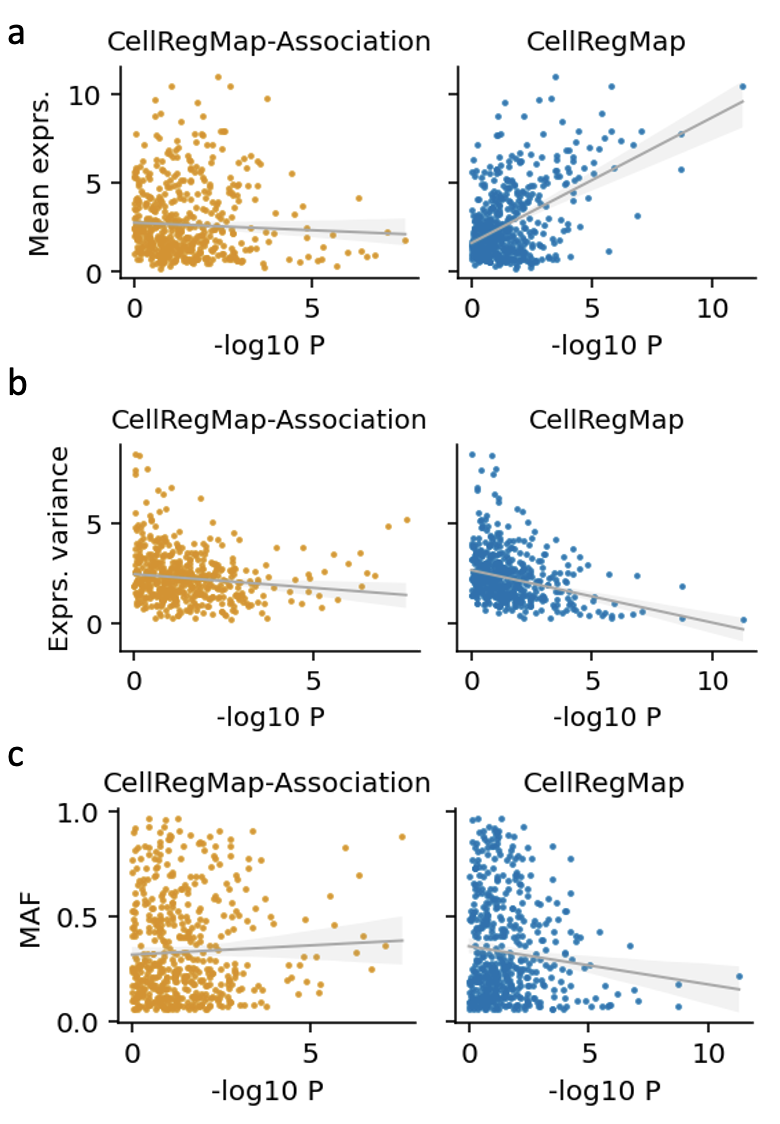
\includegraphics[width=10cm]{Appendix_CellRegMap/SuppFigures/Fig_S3.png}
    \caption{\textbf{eQTL statistics stratified for gene properties on simulated data.}
    Results for simulated genetic effects using the same parameters as in \textbf{Appendix Fig. S2} (10 MOFA factors with GxC, fraction of genetic variance explained by GxC = 0.5; \textbf{Materials and Methods}). 
    Shown are the \textbf{(a)} mean observed gene expression of the simulated eGene (prior to adding the genetic effect), \textbf{(b)} the prior gene expression variance and \textbf{(c)} the minor allele frequency as a function of the P-value estimated by CellRegMap (blue) and CellRegMap-Association (orange). 
    Both models are fitted using the same set of ground truth context variables as used in the simulation. 
    Lines show the regression fit and shaded areas 95\% confidence intervals.
}
\end{figure}

\begin{figure}[h]
    \centering
    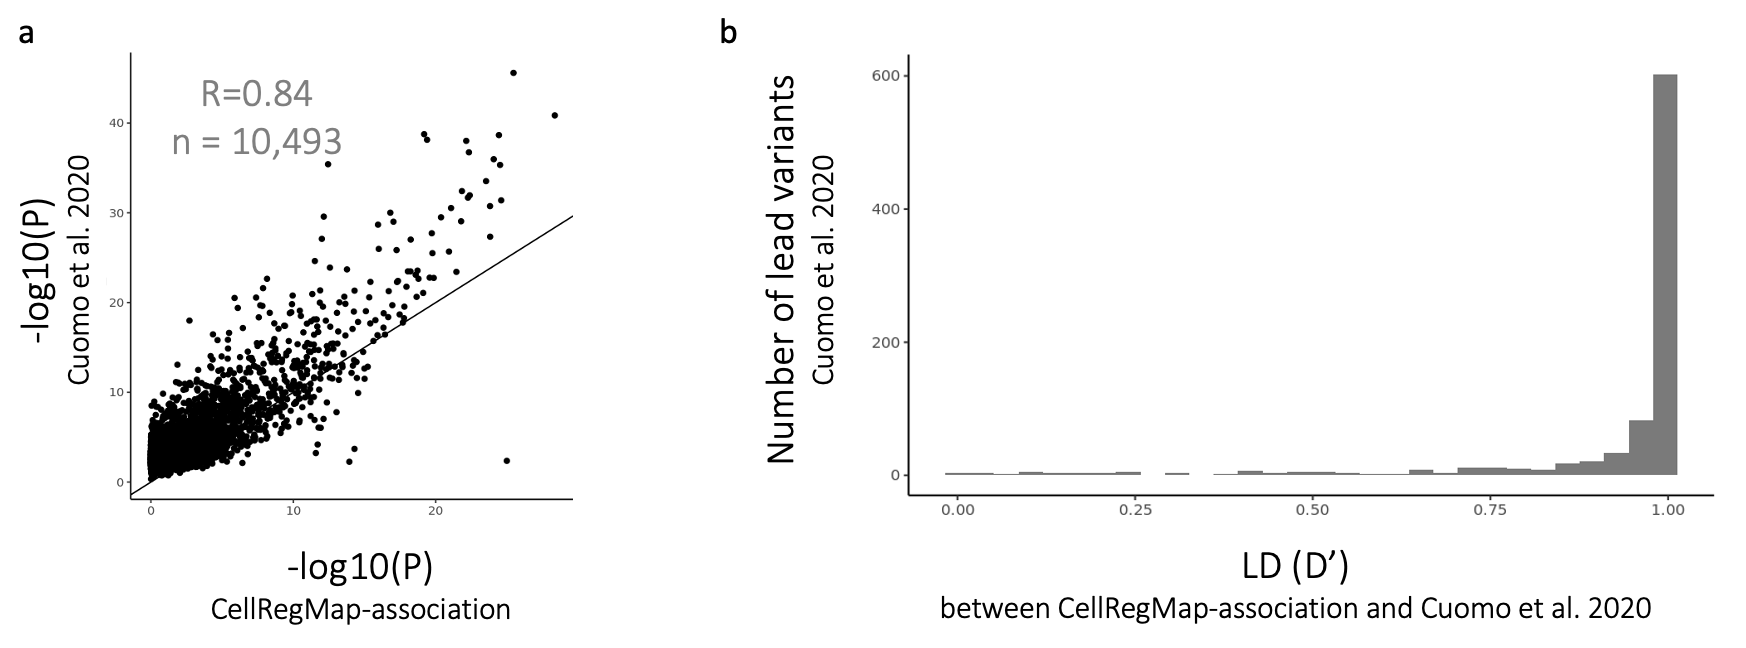
\includegraphics[width=16cm]{Appendix_CellRegMap/SuppFigures/Fig_S4.png}
    \caption{\textbf{Concordance of persistent genetic effects on endoderm differentiation data.}
    Data from \cite{cuomo2020single}. 
    \textbf{(a)} Scatter plot of -log10 p-values from the original study (\cite{cuomo2020single}, y-axis) vs -log10 p-values when using the CellRegMap-association test (x-axis). 
    For the published study, the top variant from each gene is considered (n=10,493 genes). 
    These results were achieved using aggregated “pseudocounts” from each of the three stages, and for each gene-SNP pair we are here selecting the smallest p-values between the iPSC, mesendoderm and definitive endoderm eQTL. 
    \textbf{(b)} For each of the significant eGenes from the original study (n=2,996), we assessed whether the lead variant identified was the same or in linkage disequilibrium (LD) with the lead variant identified by CellRegMap-association. 
    Histogram of the LD (D’, as calculated using the R package “LDlinkR”, \cite{myers2020ldlinkr}) distribution between lead variants from the two tests.
}
\end{figure}

\begin{figure}[h]
    \centering
    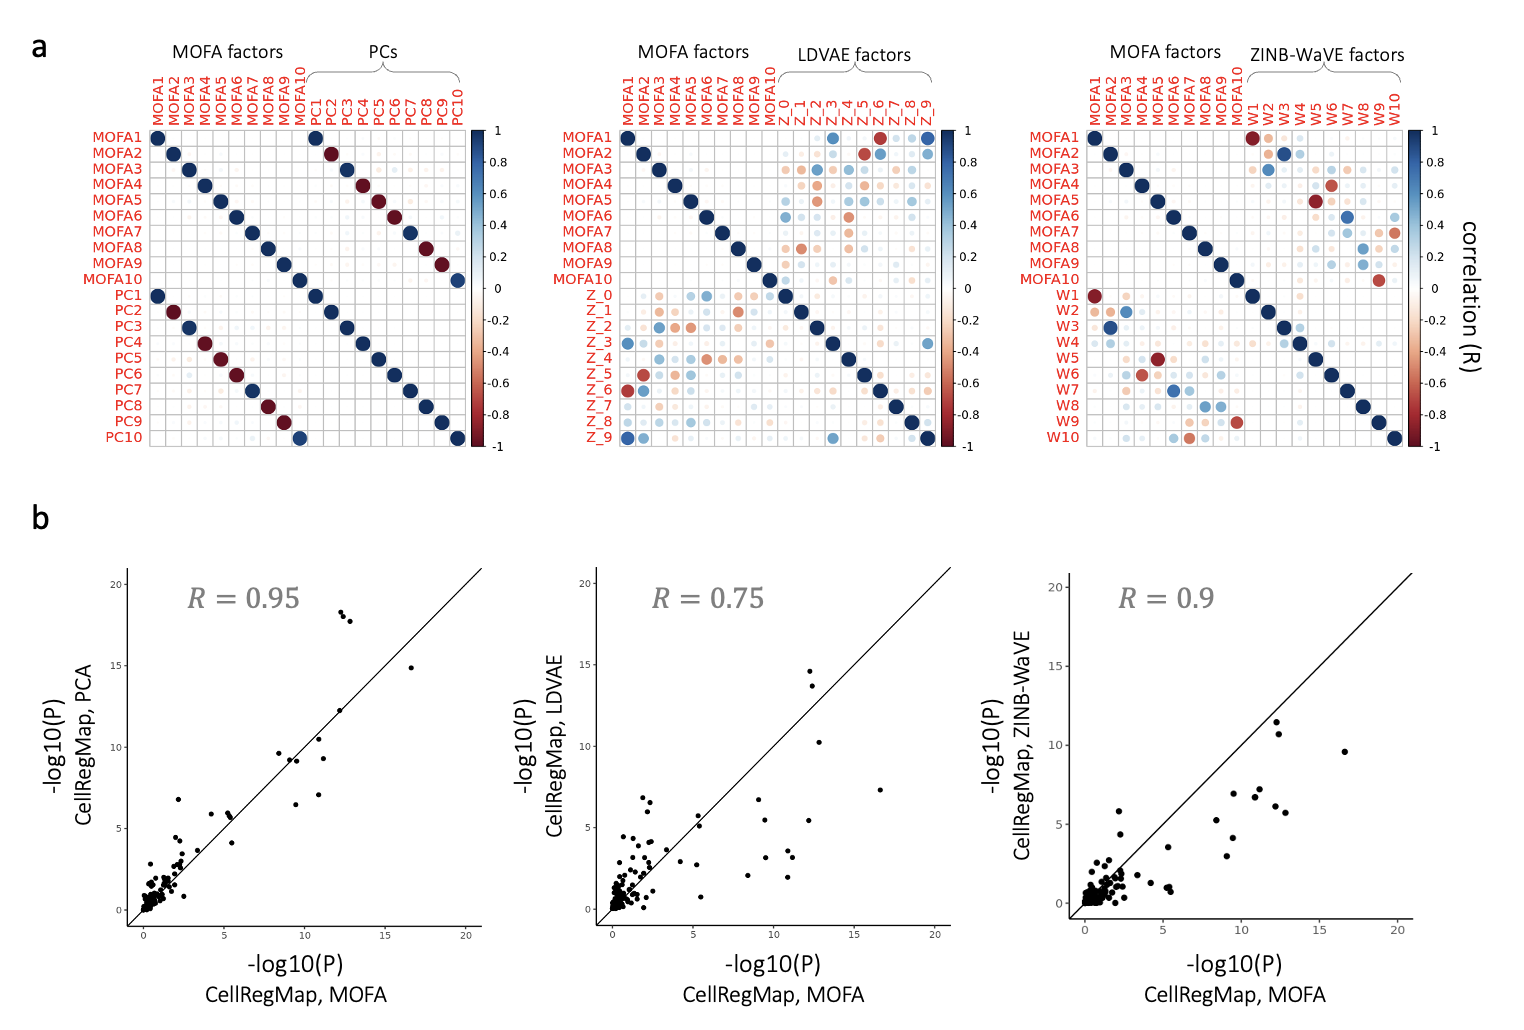
\includegraphics[width=16cm]{Appendix_CellRegMap/SuppFigures/Fig_S5.png}
    \caption{\textbf{Comparison of alternative methods to define cellular contexts.}
    Assessment based on the endoderm differentiation study \cite{cuomo2020single}. 
    We compared the MOFA workflow to define cellular contexts to principal component analysis (left), linearly-decoded variational autoencoder (LDVAE \cite{svensson2020interpretable}, middle) and zero-inflated negative binomial-based wanted variation extraction (ZINB-WaVe \cite{risso2018general}, right). 
    \textbf{(a)} Correlation matrix between the leading 10 factors identified by MOFA and the respective alternative method.  
    \textbf{(b)} Scatter plot of negative log p-value of the CellRegMap interaction test when using MOFA cell contexts (x-axis) versus using a cell-context covariance derived using the respective alternative method (y-axis). 
    Considered are n=121 SNP-gene pairs from 88 unique genes on chromosome 22 only.
}
\end{figure}

\begin{figure}[h]
    \centering
    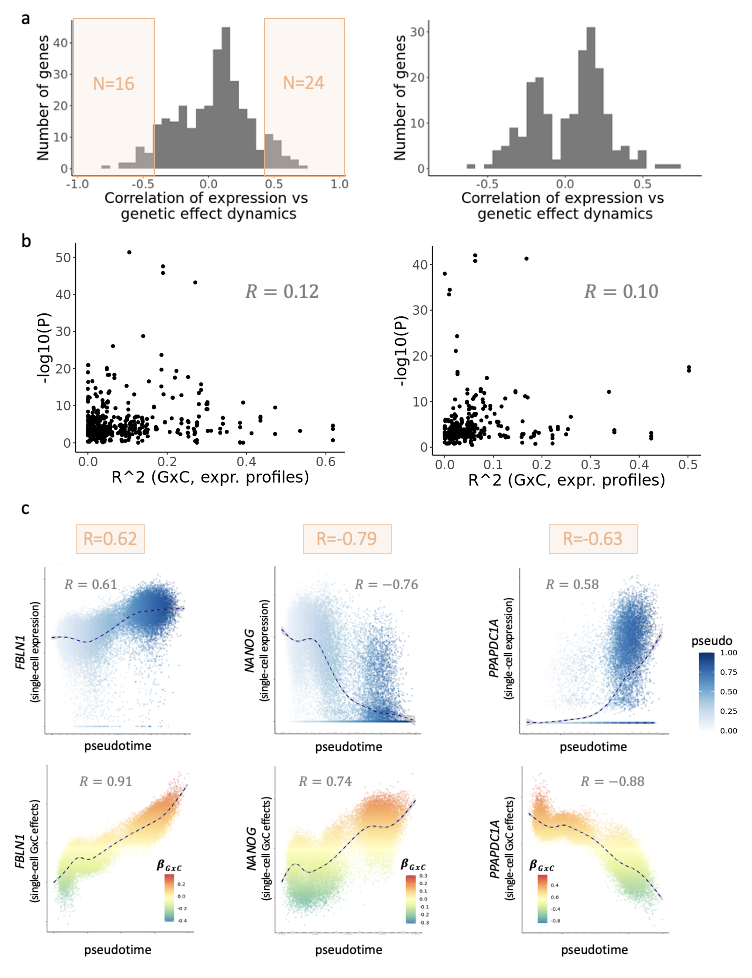
\includegraphics[width=11cm]{Appendix_CellRegMap/SuppFigures/Fig_S6.png}
    \caption{\textbf{Correlations of GxC with gene expression dynamics.}
    \textbf{(a)} Correlation (R) between single-cell expression profiles and estimated single-cell genetic effect profiles for 322 and 213 genes with significant GxC effects respectively (FDR$<$5\%) (left: endoderm differentiation data from Cuomo et al \cite{cuomo2020single}, right: neuronal differentiation data from Jerber et al \cite{jerber2021population}). 
    \textbf{(b)} Scatter plot between the R2 correlation coefficient between gene expression and GxC (x axis, as in \textbf{a}, but considering R2 instead of R) versus the statistical significance of GxC effects (-log10(p-value), y axis)  (left: endoderm differentiation data from Cuomo et al, right: neuronal differentiation data from Jerber et al). 
    \textbf{(c)} For three examples from a (high $|$R$|$ between expression and GxC effects dynamics), the top row represents single-cell expression the genes (y-axis) as a function of pseudotime (x-axis); the bottom row represents the single-cell genetic effect estimates due to GxC (y-axis) as a function of pseudotime (x-axis). 
    In orange, the R coefficient between expression and GxC effect dynamics, as in \textbf{a}.
}
\end{figure}

\begin{figure}[h]
    \centering
    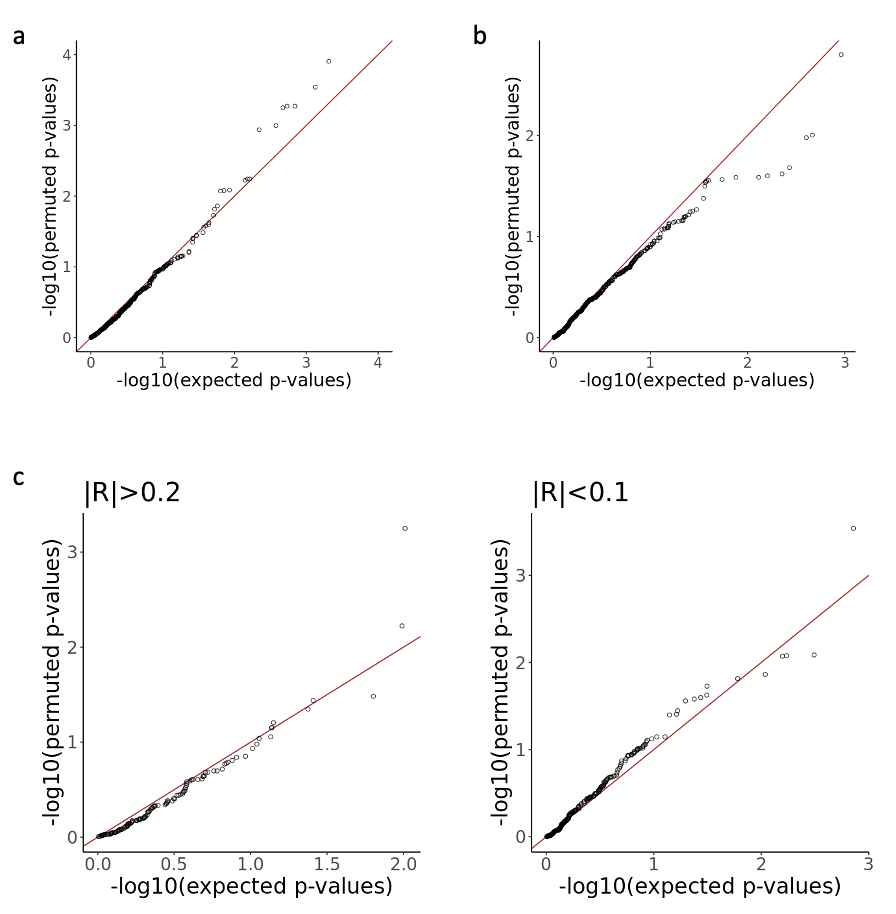
\includegraphics[width=13cm]{Appendix_CellRegMap/SuppFigures/Fig_S7.png}
    \caption{\textbf{Calibration of CellRegMap in relation to expression dynamics.}
    Shown are results obtained from the endoderm differentiation data \cite{cuomo2020single}; (GxC interaction test) considering genes on chromosome 22 only. 
    QQplots demonstrating calibration using permitted genotypes (GxC component only) \textbf{(a)} Across all gene-SNP pairs from (n=540, i.e. 270 genes, 2 SNPs each): median=0.57. 
    \textbf{(b)} Across all gene-SNP pairs from (neuron differentiation data from Jerber et al, [3]) (n=500, i.e. 250 genes, 2 SNPs each): median=0.51. 
    \textbf{(c)} Considering the endoderm differentiation data, as in a, but stratifying genes by those whose expression is (left) correlated with differentiation time ($|$R$|>$0.2; n=134, median=0.51) and (right) not correlated with differentiation time ($|$R$|<$0.1; n=218, median=0.47).
}
\end{figure}

\begin{figure}[h]
    \centering
    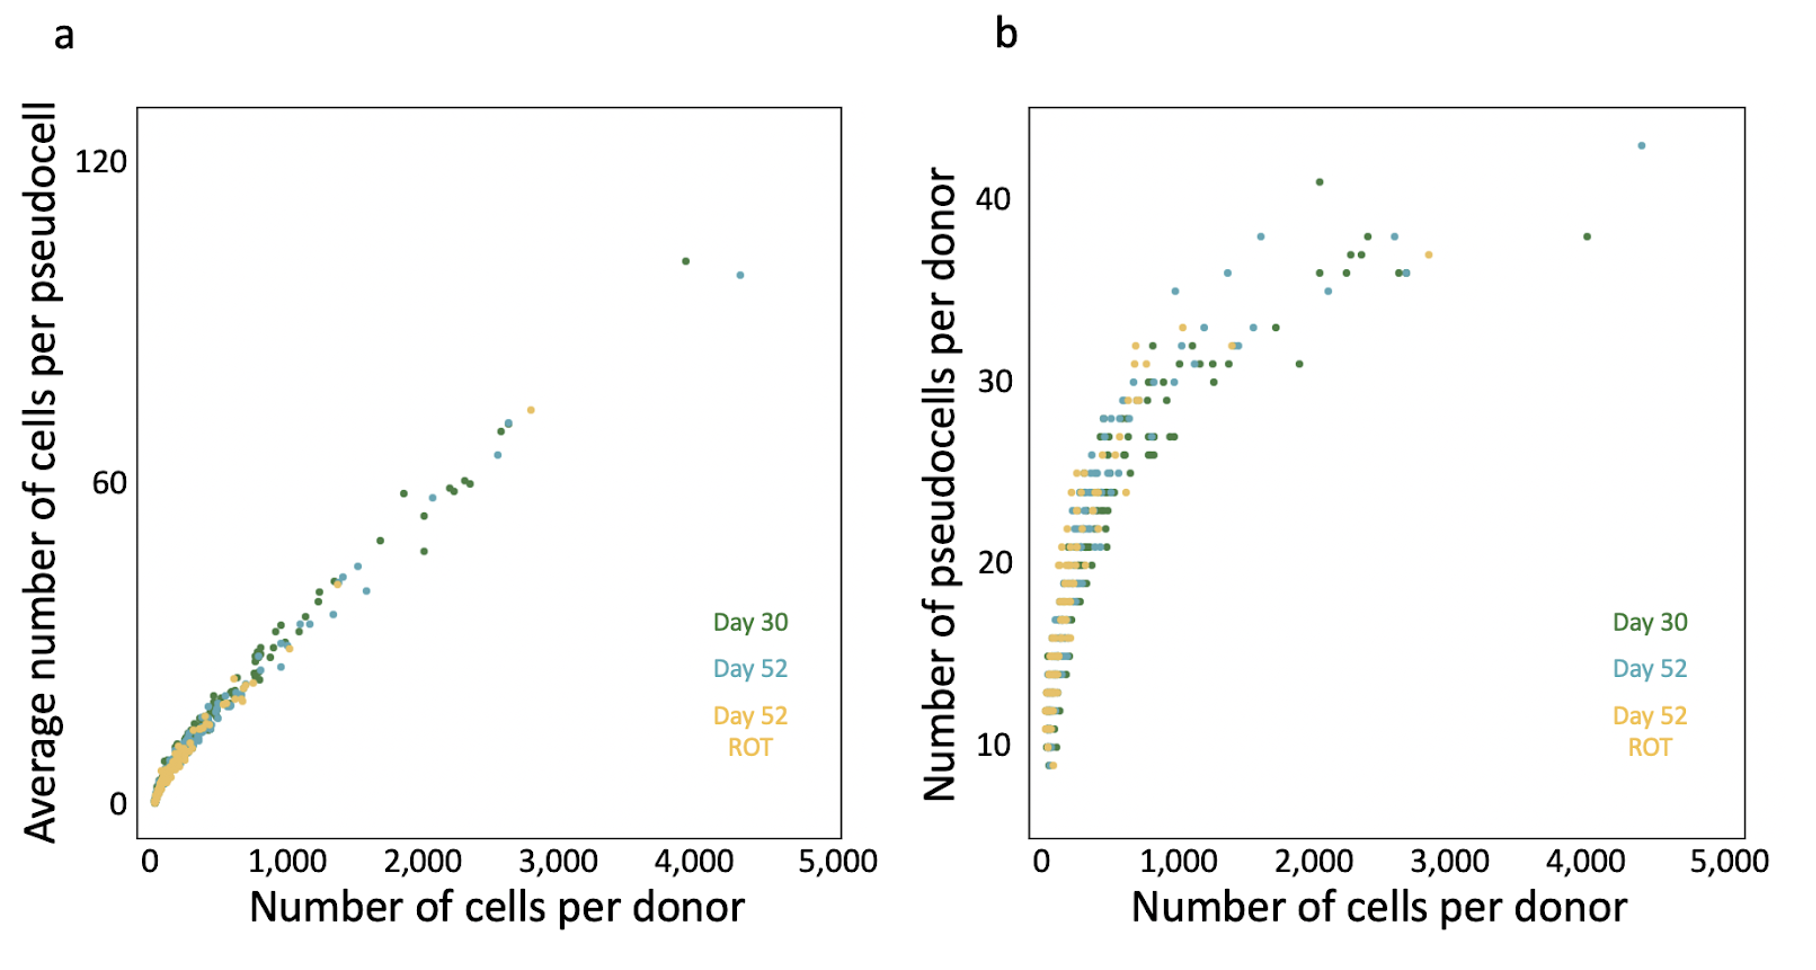
\includegraphics[width=13cm]{Appendix_CellRegMap/SuppFigures/Fig_S8.png}
    \caption{\textbf{Dopaminergic neuron pseudocell aggregation.}
    Transcriptionally related cells were aggregated into pseudocells, thereby reducing the sparsity in this dataset (dopaminergic neurons from \cite{jerber2021population}). 
    Pseudocells were constructed separately for each individual and conditions (day 30, day 52, rotenone-treated day 52; \textbf{Materials and Methods}).
    \textbf{(a)} Scatter plot between the number of cells for each individual (x axis) versus the average number of cells contained in a pseudocell for the corresponding individual (y axis). 
    Colour denotes the three main cell populations (collected across three conditions). 
    \textbf{(b)} Analogous as in a, comparing the number of cells per donor versus the number of pseudocells per donor.
}
\end{figure}


\begin{figure}[h]
    \centering
    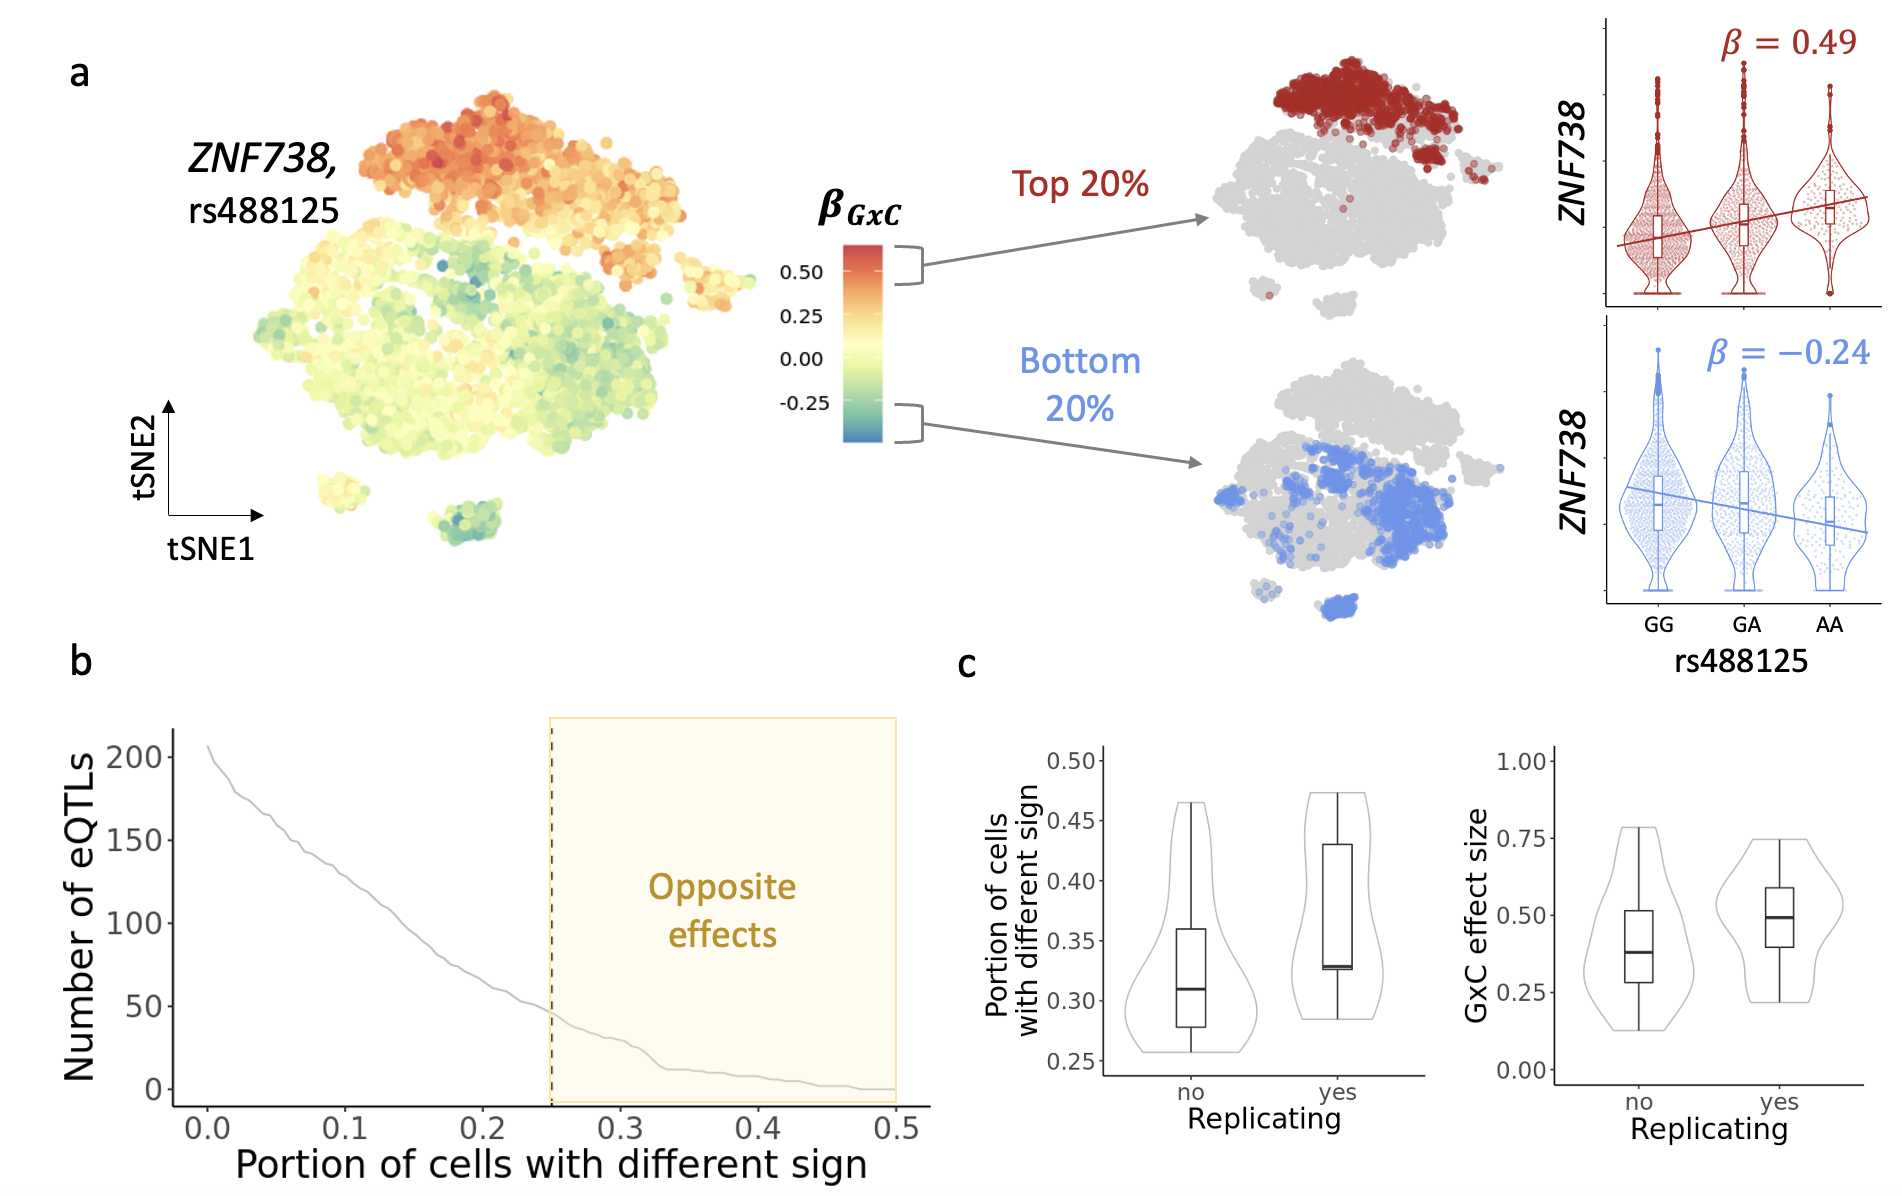
\includegraphics[width=16cm]{Appendix_CellRegMap/SuppFigures/Fig_S9.png}
    \caption{\textbf{Opposite effects detected by GxC.} 
    Considering data from \cite{cuomo2020single}. 
    \textbf{(a)} Example of “true” opposite effects. 
    The estimated genetic effects due to GxC (GxC) across all cells for the depicted eQTL (gene: \textit{ZNF738}, SNP: chr19:21474173) indicates opposite effects across different populations, as shown by the tSNE plot on the left. 
    To further assess this effect, we considered two extreme strata of cells (top and bottom 20\% of the GxC values, tSNE plots in the middle) and assessed direction of effect in each stratum using a standard eQTL mapping strategy (based on pseudo bulk mapping; \textbf{Materials and Methods}), demonstrating true opposite effects (box plots on the right). 
    \textbf{(b)} Distribution of the portion of cells with different sign from the rest in the GxC values (0 corresponds to the setting that indicates that GxC estimates for a given eQTL variant have consistent sign across all cells; 0.5 corresponds to 50\% of all cells having an opposite effect signtake on assumes only positive values across all cells only, 1 negative for all cells), for all significant GxC eQTL (n=213, FDR$<$5\%; neuronal development data). 
    We define a GxC eQTL as displaying opposite effects when at least 25\% of cells have a different sign compared to the rest in the estimated GxC values.
    \textbf{(c)} Next, we considered the 45 opposite effects from \textbf{(b)}, and assessed replication, by mapping standard eQTL when considering the top and bottom 20\% of cells (based on GxC values, as shown for the example in a). 
    When comparing the opposite effects that do replicate (opposite effect sizes using standard strategies as described in a; \textbf{Materials and Methods}) to those that do not replicate, we observe that (left) portion of cells with different signs is higher for the replicating ones (closer to a 50-50 split between positive and negative values), and (right) the estimated magnitude of GxC effect sizes (calculated as the delta of the top and bottom 10\% of GxC values) is lower for the non-replicating opposite effects.
}
\end{figure}

\begin{figure}[h]
    \centering
    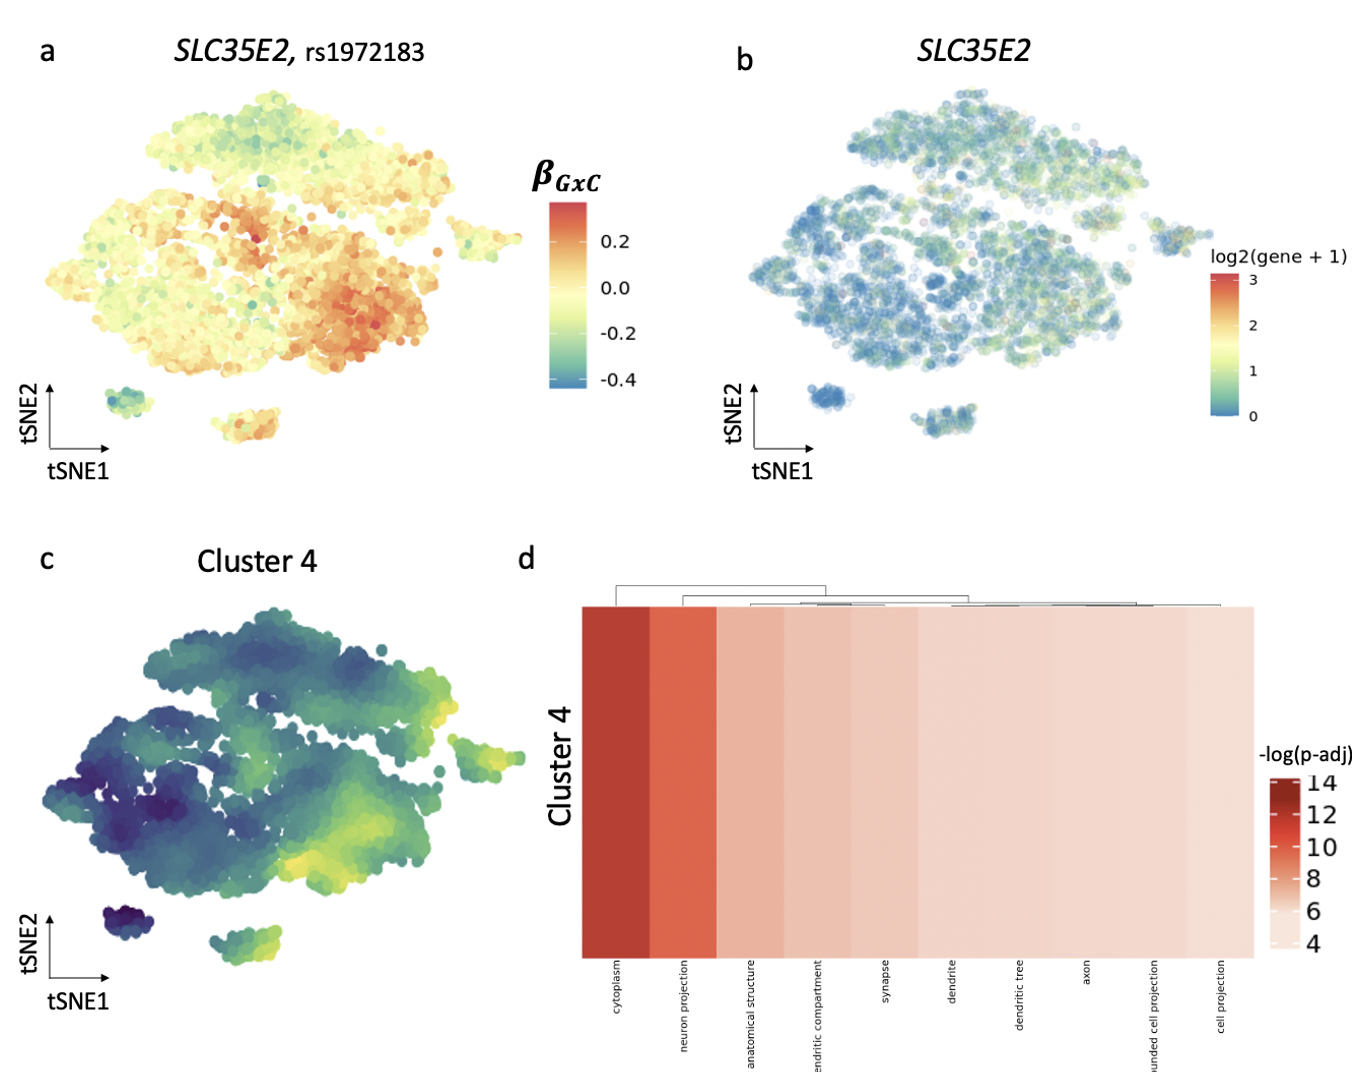
\includegraphics[width=14cm]{Appendix_CellRegMap/SuppFigures/Fig_S10.png}
    \caption{\textbf{CellRegMap to fine-map cellular context for human disease variant.} 
    Considering the subset of cells identified as dopaminergic neurons from \cite{jerber2021population}. \textbf{(a)} GxC profile at rs1972183 for \textit{SLC35E2}, which is colocalized with a GWAS variant for sleeplessness and insomnia in the subpopulation of day 52 untreated cells. 
    Shown is a scatter plot of the first two tSNE coordinates with colour denoting the estimated GxC effect component GxC. 
    \textbf{(b)} As in \textbf{a}, with colour denoting \textit{SLC35E2} single-cell gene expression levels. 
    \textbf{(c)} Manifold of consensus relative GxC effect sizes estimates for cluster 4, which contains the GxC effects for \textit{SLC35E2}.  
    \textbf{(d)} Extract of the gene enrichment analysis for cluster 4 (based on \textbf{Fig. EV4b}).
}
\end{figure}

\begin{figure}[h]
    \centering
    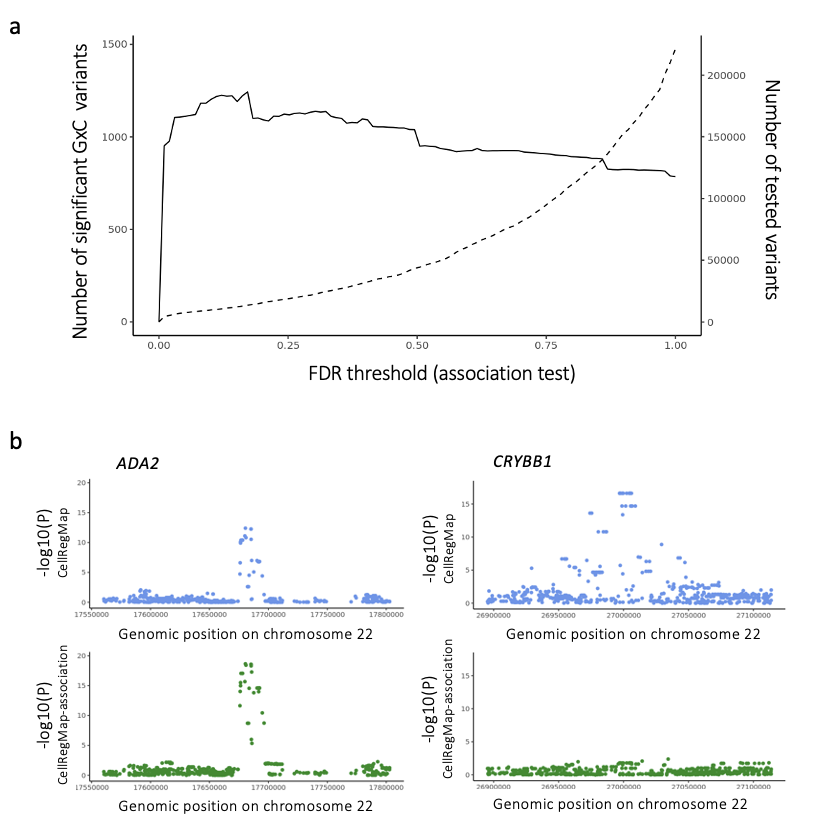
\includegraphics[width=13cm]{Appendix_CellRegMap/SuppFigures/Fig_S11.png}
    \caption{\textbf{Assessment of two-stage workflow using the CellRegMap-association test to define candidate eQTL for GxC analysis.} 
    Results based on the endoderm differentiation data \cite{cuomo2020single}, using the de-novo for both persistent effects using  the CellRegMap-association test and GxC interactions using the CellRegMap interaction test (+/- 100kb around the gene body, MAF$>$5\%, all expressed genes on chromosomes 20-22). 
    \textbf{(a)} Number of significant GxC effects (FDR$<$1\%; y-axis) as a function of the FDR threshold to filter for variants based on the association signal (x axis). 
    Second y-axis denotes the number of tested SNP-gene pairs. 
    While the number of tested SNP-gene pairs increases for less stringent filtering, the number of detected GxC effects decreases, indicating that no discoveries are lost when considering the top eQTL only, while computation time is saved, and power to find GxC is also (slightly) increased. 
    \textbf{(b)} Manhattan plots representing examples of same (left, for the \textit{ADA2} gene) vs different (right, for the \textit{CRYBB1} gene) signals being picked up by CellRegMap’s GxC interaction test (blue) and CellRegMap association test (green).
}
\end{figure}
% \section{Supplementary Methods}
\section{The CellRegMap model}\label{sec:CellRegMap} 

CellRegMap builds on and extends the structured linear mixed model (StructLMM \cite{moore2019linear}), which has recently been proposed to test for genotype-environment interactions on physiological traits in population cohorts. 
CellRegMap extends this model to test for interactions between genotype and cellular context on gene expression using single-cell RNA-seq as readout. 
The model is not designed for variant discovery but instead designed to identify and characterize genotype-context (G$\times$C) interactions at known expression quantitative trait loci (eQTL).
However, if eQTL are not known \textit{a priori}, it is possible to run the Association test implemented within the CellRegMap software, in order to identify candidate eQTL to test for G$\times$C interactions (section~\ref{sec:assoc}).
In Section~\ref{sec:model}, the CellRegMap model is motivated and derived, followed by the introduction of an efficient scheme for parameter inference and statistical testing.
Section~\ref{sec:assoc} describes the association test implemented within CellRegMap, while section~\ref{sec:beta_gxe} describes the procedure to estimate cell-level effect sizes due to G$\times$C.

\subsection{Model definition}
\label{sec:model}
% clarify that samples (N) are cells (or pseudocells)
% maybe start directly from structLMM (not LM, LMM)

Commonly used methods for eQTL mapping based on linear or linear mixed models (LMM) relate individual genetic variants to the expression level of a gene of interest, \textit{i.e.},
% \begin{equation}\label{eq:LM}
%  \mathbf{y} =  \mathbf{W}\boldsymbol{\alpha} + \mathbf{g}\beta_G + \boldsymbol{\psi},
% \end{equation}

\begin{equation}\label{eq:LMM}
 \mathbf{y} =  \mathbf{W}\boldsymbol{\alpha} + \mathbf{g}\beta_G + \boldsymbol{\psi}. 
\end{equation}

Here, $\mathbf{y}$ denotes a $N \times 1$ vector of the expression level of a gene of interest across $N$ individuals (typically measured using bulk RNA sequencing); $\mathbf{W}$ is the $N \times P$ design matrix of covariates and $\alpha_i, i=1,..,P$ are the corresponding weights (note that in the main text, \textit{i.e.}, \textbf{Figure 1d}, covariates are omitted for brevity); $\mathbf{g}$ is the $N \times 1$ vector of alleles for each individual at the locus to be assessed and $\beta_G$ denotes the corresponding effect size.
% The variable $\mathbf{u}$ denotes a random effect term, which can be used to account for additive confounding factors or relatedness, and f
Finally, $\boldsymbol{\psi}$ denotes i.i.d. noise, $\boldsymbol{\psi} \sim \mathcal{N}(\mathbf{0}, \sigma_n^2\mathbf{I})$.
Additional random effect components have been introduced to account for relatedness between individuals~\cite{hoffman2013correcting}, or to adjust for additive confounding sources of variation on gene expression~\cite{fusi2012joint}. 
% \\

\subsubsection*{Review of StructLMM}
StructLMM \cite{moore2019linear} extends the conventional linear association test in Eq.~\eqref{eq:LMM} by including an additional random effect component to account for heterogeneity in effect sizes across individuals due to context-specific genetic effects. 
Briefly, StructLMM can be cast as:

\begin{equation}\label{eq:StructLMM}
 \mathbf{y} =  \mathbf{W}\boldsymbol{\alpha} + \mathbf{g}\beta_G + \mathbf{g} \odot \boldsymbol{\beta_{GxC}} + \mathbf{c} +\boldsymbol{\psi}, 
\end{equation}

where $\mathbf{g} \odot \boldsymbol{\beta_{GxC}}$ accounts for G $\times$ C and $\mathbf{c}$ for additive contributions of environmental variation. 
Unlike in conventional interaction tests, genotype-context interactions due to environmental variation are accounted by introducing an additional genetic effect with per-individual effects, where each individual has its own effect size.
The symbol $\odot$ denotes the Hadamard product and $\boldsymbol{\beta_{GxC}}=[\beta_{GxC_1}, .. ,\beta_{GxC_N}]^T$ is a vector of per-individual effect sizes to account for heterogeneous genetic effects.
Instead of explicitly estimating the GxC effect sizes, these parameters are marginalised under a multivariate normal prior distribution that is defined by an environmental context covariance matrix:

\begin{equation}\label{eq:beta_GxE}
    \boldsymbol{\beta_{GxC}} \sim \mathcal{N}(\mathbf{0},\sigma_{GxC}^2 \boldsymbol{\Sigma}).
\end{equation} 

In this case the covariance $\boldsymbol{\Sigma}$ does not encode relatedness as in a classical LMM, but instead accounts for sample covariance due to different environmental states.
The same environmental covariance matrix can also be used to parametrize a second random effect component to account for additive environmental contributions,

\begin{equation}
   \mathbf{c} \sim \mathcal{N}(\mathbf{0},\sigma_c^2 \boldsymbol{\Sigma}). 
\end{equation}

Notably, StructLMM does not account for any additional structure across samples, such as population structure or repeat measurements.
While discrete populations can be accounted for as covariates, more subtle relatedness or repeat structure cannot be effectively encoded using fixed effect covariates. 
Consequently, the model is not suitable for any experimental design where multiple observations are available for the same individual, which is the case in single-cell genetic studies, where multiple cells are assayed from each individual. 
Such a repeat structure results in un-calibrated p-values; see also the results from the simulation study to assess calibration (main text \textbf{Fig. 2}). 
% \\

\subsubsection*{CellRegMap}
CellRegMap extends StructLMM to allow for applications to single-cell expression data by introducing an additional random effect component that accounts for relatedness or sample repeat structure. 
First, we note that the phenotype $\mathbf{y}$ now represents single-cell resolved expression data, so our samples are expression levels in cells, not individuals. 
This introduces additional structure in the data, as typically multiple cells are sampled from the same individual.
To account for this structure, an additional random effect component $\mathbf{u}$ is included in the model: 

\begin{equation}\label{eq:scStructLMM}
 \mathbf{y} =  \mathbf{W}\boldsymbol{\alpha} + \mathbf{g}\beta_G + \mathbf{g} \odot \boldsymbol{\beta_{GxC}} + \mathbf{c} + \mathbf{u} + \boldsymbol{\psi}. 
\end{equation}

Here, $\mathbf{y}$ has the cardinality of single-cells rather than individuals, and hence the G$\times$C component ($\mathbf{g} \odot \boldsymbol{\beta_{GxC}}$) accounts for interactions with cellular states and contexts (which are well defined at the level of single cells) as well as environmental exposures and stimuli (which can also be individual-level).
The terms $\mathbf{c} \sim \mathcal{N}(\mathbf{0},\sigma_c^2 \boldsymbol{\Sigma})$ and $\boldsymbol{\psi} \sim \mathcal{N}(\mathbf{0},\sigma_n^2\mathbf{I})$ have the same meaning as previously, noting that for these $N \times 1$ vectors $N$ now represents the total number of cells, not the number of unique individuals.
Similarly, $\boldsymbol{\Sigma})$ is $N \times N$ and is again defined in the space of cells.
The symbol $\boldsymbol{\beta_{GxC}}\sim \mathcal{N}(\mathbf{0},\sigma_{GxC}^2 \boldsymbol{\Sigma})$ now represents cell-level effect sizes, which again captures variation in genetic effects across cells.
% to account for heterogeneous genetic effects, which follows a multivariate normal distribution:
% \begin{equation}\label{eq:beta_GxE}
%     \boldsymbol{\beta_{GxE}} \sim \mathcal{N}(\mathbf{0},\sigma_{GxE}^2 \boldsymbol{\Sigma}),
% \end{equation}
% Depending on the functional form of the environmental covariance $\boldsymbol{\Sigma}$, this model can account for different types of G$\times$E, for example, both discrete and continuous cell states and types or donor-level environmental covariates. 
% The same environmental covariance matrix is also used to account for additive environmental effects:
% \begin{equation}
%   \mathbf{e} \sim \mathcal{N}(\mathbf{0},\sigma_e^2 \boldsymbol{\Sigma}). 
% \end{equation}
% Finally, the model includes a background term that accounts for interactions of repeat structure ($\mathbf{R}$) and environments ($\boldsymbol{\Sigma}$):
The additional random effect component $\mathbf{u}$ accounts for relatedness or the repeat structure, which is parametrized as a product kernel between relatedness ($\mathbf{R}$) and the environmental covariance ($\boldsymbol{\Sigma}$):

\begin{equation}
    \mathbf{u} \sim \mathcal{N}(\mathbf{0},\sigma_{rc}^2 \mathbf{R} \odot \boldsymbol{\Sigma}).
\end{equation}

Here, $\mathbf{R}$ denotes the relatedness matrix of individuals expanded to all cells based on the known assignment of cells to individuals and the covariance $\mathbf{\Sigma}$ again denotes the cell-level environmental context.
Notably, this parametrization extends the classical LMM, which would exclusively consider a relatedness component $\mathbf{R}$.
One way to interpret this covariance is to account for polygenic interactions between environmental and relatedness, which has previously been considered to estimate the GxE component of heritability~\cite{heckerman2016linear}.


% Finally, we include a background term ($\mathbf{u}$) to model non-random interactions between the repeat structure and such contexts. 

% where we note that $\mathbf{R}$ is appropriately expanded to reflect the repeated structure of multiple cells derived from the same individuals. 

\subsection{Construction of the cellular context covariance}

Typically, we define $\boldsymbol{\Sigma} = \mathbf{E}\mathbf{E}^T$, and hence the cellular context covariance is a linear function of a matrix of environmental states $\mathbf{E}$.
In practice, we consider as cellular contexts axes of variation in the dataset (for example captured by principal components or MOFA \cite{argelaguet2018multi} factors), appropriately standardized (mean=0, standard deviation=1) and build $\boldsymbol{\Sigma} = \mathbf{E}\mathbf{E}^T$ accordingly.
Depending on the type and structure of cellular contexts, $\boldsymbol{\Sigma}$ can simply separate cells into groups, and appear as a block diagonal or capture continuous transitions (main text \textbf{Fig. 1c}). 
In principle, CellRegMap can also be use in conjunction with other parametrizations of the cell context covariance.

\subsection{Statistical testing}

The main operations in the CellRegMap model, including parameter inference and tests are implemented in its marginalised form. 
Integrating over the random effect components, the marginal likelihood of the model in Eq. \eqref{eq:scStructLMM} follows as:

\begin{equation}
    \label{eq:scStructLMM_marginal}
     \mathbf{y} \sim \mathcal{N} ( \mathbf{W}\boldsymbol{\alpha} + \mathbf{g}\beta_G, \sigma^2_{GxC} \text{diag}(\mathbf{g}) \boldsymbol{\Sigma} \text{diag}(\mathbf{g}) + \sigma_c^2 \boldsymbol{\Sigma} + \sigma_{rc}^2 \mathbf{R} \odot \boldsymbol{\Sigma}+ \sigma_n^2 \mathbf{I} ). 
\end{equation}

While in principle CellRegMap can be used to test for different components, including additive genetics, interactions or the combination of both effects (see~\cite{moore2019linear} for details on StructLMM), we here focus on GxC effects. 
In order to evaluate the significant contribution of GxC effects, we consider a statistical test that compares the following hypotheses, from Eq.\eqref{eq:scStructLMM}:

\begin{equation*}
    H_0: \sigma_{GxC}^2 = 0,
\end{equation*}

\begin{equation*}
    H_1: \sigma_{GxC}^2 > 0.
\end{equation*}

We use Rao's Score test~\cite{rao1948large} to evaluate significance, which allows us to only calculate the MLE\footnote{maximum likelihood estimator} of the parameters under the null hypothesis $H_0$, which follows from~Eq.\eqref{eq:scStructLMM_marginal} as:

\begin{equation}\label{eq:scStructLMM_H0_MVN}
 \mathbf{y}|H_0 \sim \mathcal{N}( \mathbf{W}\boldsymbol{\alpha} + \mathbf{g}\beta_G, \sigma_c^2 \boldsymbol{\Sigma} + \sigma_{rc}^2 \mathbf{R} \odot \boldsymbol{\Sigma}+ \sigma_n^2 \mathbf{I} ). 
\end{equation}
% \\

To test for GxC interactions we adapt the score-based testing scheme employed in StructLMM, which in turn adopts fast LMM testing in LMMs as first proposed in Lippert et al., \cite{lippert2011fast}.
We here review the key steps involved.
\\

First, we define the score-based test statistic $\mathrm{Q}$ as:

\begin{equation}\label{eq:Q}
    \mathrm{Q} = \frac{1}{2}\mathbf{y}^T\mathbf{P}_0 \frac{\partial \mathbf{K}}{\partial \theta}\mathbf{P}_0 \mathbf{y}, 
\end{equation}

where $\mathbf{K}$ denotes the full covariance matrix, \textit{i.e.}, from Eq. \eqref{eq:scStructLMM}:

\begin{equation}\label{eq:full_K_scStructLMM}
    \mathbf{K} = \sigma_{GxC}^2\mathrm{diag}(\mathbf{g})\boldsymbol{\Sigma} \ \mathrm{diag}(\mathbf{g}) +  \sigma_c^2 \boldsymbol{\Sigma} + \sigma_{rc}^2 \mathbf{R}\odot\boldsymbol{\Sigma}+ \sigma_n^2 \mathbf{I},
\end{equation}

and 

\begin{equation}
    \mathbf{P}_0 = \mathbf{K}_0^{-1}-\mathbf{K}_0^{-1}\mathbf{X}(\mathbf{X}^T\mathbf{K}_0^{-1}\mathbf{X})^{-1}\mathbf{X}^T\mathbf{K}_0^{-1}
\end{equation}

is a matrix that projects out the fixed effects \cite{lippert2011fast, lippert2014greater}.
In our case (Eq.\eqref{eq:scStructLMM}), the fixed effects include covariates and the persistent effect of the variant tested: $\mathbf{X} = [\mathbf{W}, \mathbf{g}]$, and $\mathbf{K}_0$ is as in Eq.\eqref{K0}.
Using Eq.\eqref{eq:full_K_scStructLMM} and considering the parameter $\theta = \sigma_{GxC}^2$, we can derive:

% \begin{equation}
%     \frac{\partial \mathbf{K}}{\partial \sigma_{GxE}^2} = \mathrm{diag}(\mathbf{g})\mathbf{E}\mathbf{E}^T\mathrm{diag}(\mathbf{g}).
% \end{equation}

% Next, let us define $\mathbf{K}_1 = \mathrm{diag}(\mathbf{g})\mathbf{E}\mathbf{E}^T\mathrm{diag}(\mathbf{g})$and substituting in eq. \eqref{eq:Q}, we can write:

\begin{equation}
    \frac{\partial \mathbf{K}}{\partial \sigma_{GxC}^2} = \mathrm{diag}(\mathbf{g})\boldsymbol{\Sigma} \ \mathrm{diag}(\mathbf{g}).
\end{equation}

Next, let us define $\mathbf{K}_1 = \mathrm{diag}(\mathbf{g})\boldsymbol{\Sigma} \ \mathrm{diag}(\mathbf{g})$; substituting in Eq.\eqref{eq:Q}, we can write:

\begin{equation}
    \mathrm{Q} = \frac{1}{2}\mathbf{y}^T\mathbf{P}_0 \mathbf{K}_1\mathbf{P}_0 \mathbf{y}. \\
\end{equation}

% \newpage

As before, $H_1: \sigma_{GxC}^2>0$, noting that as a variance parameter, $\sigma_{GxC}^2$ is constrained to take on positive values.
As a result, the score test statistic $\mathrm{Q}$ follows a mixture of $\chi^2$ distributions\footnote{We refer the reader specifically to the supplementary methods from \cite{lippert2014greater} for a proof.}:

\begin{equation}
    \mathrm{Q} \sim \sum_i \lambda_i \chi^2_1, 
\end{equation}

where $\lambda_i$'s are the non-zero eigenvalues of $\frac{1}{2}\mathbf{P}_0^{\frac{T}{2}} \frac{\partial\mathbf{K}}{\partial \theta} \mathbf{P}_0^{\frac{1}{2}}$.\\

It can be shown that for a matrix $\mathbf{A}$ the non-zero eigenvalues of $\mathbf{A}\mathbf{A}^T$ are the same as those of $\mathbf{A}^T\mathbf{A}$ , thus we can re-arrange and compute $\lambda_i$'s as the eigenvalues of:

\begin{equation}
    \frac{1}{2}\frac{\partial\mathbf{K}}{\partial \theta}^{\frac{T}{2}} \mathbf{P}_0 \frac{\partial\mathbf{K}}{\partial \theta}^{\frac{1}{2}}
\end{equation}

instead. 
% \\
To evaluate the significance of the score-best test statistic $\mathrm{Q}$ we use the approach described in Sequence Kernel Association Test (SKAT \cite{wu2011rare}), thereby using the Davies exact method \cite{davies1980algorithm} to compute the corresponding p values, and switching to the modified moment matching approximation method \cite{liu2009new, lee2012optimal, duchesne2010computing} when this fails to converge.

\subsection{Implementation}

To enable efficient parameter inference, we extended the strategy in StructLMM~\cite{moore2019linear}, which builds on the reparametrization of the LMM likelihood proposed in~\cite{lippert2011fast}. 
Briefly, the key is to rewrite the overall covariance of $\mathbf{y}|H_0$ in the form: $\sigma^2_m(\mathbf{M}+\delta\mathbf{I})$, where $\mathbf{M}$ is ideally low rank to enable an efficient singular value decomposition.  
To do so, we introduce a weight parameter $\rho_1$, such that the covariance matrix of $\mathbf{y}$ under the null hypothesis, $\mathbf{K}_0 = \mathrm{Cov}(\mathbf{y} | H_0)$ can be cast as:

\begin{equation}\label{K0}
\begin{split}
    \mathbf{K}_0 = \sigma_c^2 \boldsymbol{\Sigma} + \sigma_{rc}^2 \mathbf{R} \odot \boldsymbol{\Sigma}+ \sigma_n^2 \mathbf{I} =\\
    \sigma_m^2 \ [\rho_1\boldsymbol{\Sigma} + (1-\rho_1) \mathbf{R} \odot \boldsymbol{\Sigma}] + \sigma_n^2 \mathbf{I} =\\ \sigma_m^2 \{ {\mathbf{M}(\rho_1) + \delta_1 \mathbf{I}\}},
\end{split}
\end{equation}

where $\sigma_m^2\rho_1 = \sigma_c^2$,
$\sigma_m^2(1-\rho_1) = \sigma_{rc}^2$,
$\delta_1 = \sigma_n^2/\sigma_m^2$, and $\mathbf{M}(\rho_1) = \rho_1\boldsymbol{\Sigma} + (1-\rho_1) \mathbf{R} \odot \boldsymbol{\Sigma}$.\\

We note that $\mathbf{M}$ only depends on $\rho_1$. 
The parameter $\rho_1$ is optimized using a grid search with values in the range 0 to 1, selecting the value of $\rho_1$ that maximises the likelihood of $\mathbf{y}|H_0$ under the null.
Once $\rho_1$ is fixed, the decomposition of $\rho_1\boldsymbol{\Sigma} + (1-\rho_1) \mathbf{R} \odot \boldsymbol{\Sigma}$ can be found using the observation that the decomposition of the linear combination of two square symmetric matrices, \textit{e.g.,}:

\begin{equation}
    \mathbf{M} = a\mathbf{A} + b\mathbf{B}
\end{equation}

can be found as a function of the decomposition of the two original matrices, \textit{i.e.,}:

\begin{equation}
    \mathbf{N} = [\sqrt{a}\mathbf{C} | \sqrt{b}\mathbf{D}]
\end{equation}

such that $\mathbf{M}=\mathbf{N}\mathbf{N}^T, \mathbf{A}=\mathbf{C}\mathbf{C}^T$ and $\mathbf{B}=\mathbf{D}\mathbf{D}^T$. 
In our case, $\mathbf{A} = \boldsymbol{\Sigma}$ and $\mathbf{B} = \mathbf{R} \odot \boldsymbol{\Sigma}$.
If $\boldsymbol{\Sigma} = \mathbf{E}\mathbf{E}^T$, its decomposition is straight-forward, with $\mathbf{C} = \mathbf{E}$.
The decomposition of the second term ($ \mathbf{R} \odot \boldsymbol{\Sigma}$), assuming $\boldsymbol{\Sigma} = \mathbf{E}\mathbf{E}^T$ and $\mathbf{R} = \mathbf{G}\mathbf{G}^T$ is a bit less trivial.
Assuming that the rank of $\mathbf{R}$ is the number of individuals, that the rank of $\boldsymbol{\Sigma}$ is the number of environments, and that the latter is smaller than the former, we can obtain $\mathbf{D}$ as the decomposition of $\mathbf{R} \odot \boldsymbol{\Sigma}$ by:

\begin{equation}
    \mathbf{R} \odot \boldsymbol{\Sigma} = \mathbf{R} \odot \sum_i[\mathbf{v}_i \lambda_i \mathbf{v}_i^T] = \sum_i[\textcolor{red}{\mathbf{R} \odot (\mathbf{v}_i \lambda_i \mathbf{v}_i^T)}].
\end{equation}

% \newpage

The terms in the sum can be rewritten as:

\begin{equation}\label{eq:Lk}
    \begin{split}
        \textcolor{red}{\mathbf{R} \odot (\mathbf{v}_i \lambda_i \mathbf{v}_i^T)} 
        & = \mathbf{R} \odot (\mathbf{u}_i \mathbf{u}_i^T) \\
        & = \mathbf{R} \odot (\mathrm{diag}(\mathbf{u}_i) \mathbf{e} \mathbf{e}^T \mathrm{diag}(\mathbf{u}_i)) \\
        & = \mathrm{diag}(\mathbf{u}_i)[\mathbf{R} \odot \mathbf{e} \mathbf{e}^T] \mathrm{diag}(\mathbf{u}_i) \\
        & = \mathrm{diag}(\mathbf{u}_i) \mathbf{R} \mathrm{diag}(\mathbf{u}_i) \\
        & = \mathrm{diag}(\mathbf{u}_i) \mathbf{G} \mathbf{G}^T  \mathrm{diag}(\mathbf{u}_i)  \\
        & = \textcolor{red}{\mathbf{Lk}_i \mathbf{Lk}_i^T},
    \end{split}
\end{equation}

where $\mathbf{Lk}_i = \mathrm{diag}(\mathbf{u}_i) \mathbf{G}$; $\lambda_i$'s and $\mathbf{v}_i$'s are eigenvalues and eigenvectors of $\mathbf{E}\mathbf{E}^T$; $\mathbf{u}_i = \sqrt{\lambda_i}\mathbf{v}_i$ and $\mathbf{e}$ is a vector of ones ($\mathbf{e} = [1..1]$). \\

% \newpage

Thus, $\mathbf{M} = \boldsymbol{\Sigma} + \mathbf{R} \odot \boldsymbol{\Sigma}$ can be written as the following sum:

\begin{equation}
    \mathbf{M} = \boldsymbol{\Sigma} + \sum_i \mathbf{Lk}_i \mathbf{Lk}_i^T,  
\end{equation}

from which follows:

\begin{equation}
    \mathbf{N} = [\mathbf{E} \ | \mathbf{Lk}_1 \ | .. \ | \mathbf{Lk}_{ne}],
\end{equation}

where $ne$ is the number of contexts considered (and the rank of $\boldsymbol{\Sigma}$).

% \newpage

% \subsection{Computational complexity}
% From using the implementation described above, it follows that the complexity is O(N) where N is the minimum between the number of cells and the product of number of unique individuals $\times$ the number of cellular contexts. Runtimes were also evaluated empirically, using simulated phenotypes for one gene, 25 SNPs and 20 different contexts (see section \ref{sec:simulations}). We considered 25 and 50 individuals, respectively, and assessed computational runtimes as a function of the number of cells per individual (25, 50, 75, 100, 125, 150) using a 2018 MacBook Pro with 2,3 GHz Quad-Core Intel Core i5 processor (Supp. Fig. 1.1).


% Various methods have been proposed to compute the tail probability of the mixture of 1-dof $\chi^2$ distributions. 
% For example, we can use the Davies method \cite{davies1980algorithm}, the moment‐matching‐based noncentral $\chi^2$ approximation method \cite{liu2009new, lee2012optimal}, or the saddlepoint approximation method \cite{kuonen1999miscellanea}. 
% The Davies methos is the most accurate but can be be computationally expensive.
% The moment-matching approximation is anti-conservative and could lead to inflated type I errors especially for small significance levels.
% SKAT: Davies + Liu
% SKATh: Davies + saddle
% \cite{wu2016efficient}

% \section{Definition of covariance matrix}

% E?

% PCs, MOFA, HVGs?
% transformation?
% normalisation/scaling

% \begin{figure}[h]
% \centering
% \includegraphics[width=15.5cm]{Chapter6/Fig/sc_structlmm_calibration.png}
% \caption[Calibration QQ-plots]{\textbf{Calibration QQ-plots}.\\
% (a) No genetic effect at all.
% (b) No GxE effect (persistent only).}
% \label{fig:sc_structlmm_calibration}
% \end{figure}

% \subsection{Comparison with StructLMM v0}

% Next, we compared our model to the original StructLMM model \cite{moore2019linear}.
% StructLMM is expected to have issues in the presence of extended repeated structure, which it is not equipped to deal with.
% To address this, we simulated various numbers of repeats per donor - mimicking cells -  ranging from 10 to 500.
% Indeed, we observe over-inflation of StructLMM in the presence of many repeats making the model not calibrated (Fig. Xa).
% sc-StructLMM, on the other hand, is nicely calibrated (Fig. Xb).

% \subsection{Comparison with standard interaction test}

% We then performed power analysis when comparing our model with one where the environments are modelled as fixed effects (see Section 2.4.2).

% % \clearpage

% \section{Application to differentiating iPS cells}

% % Next, 
% I applied sc-StructLMM on the data described in \textbf{Chapter 
% % \ref{chapter4}
% 4} (and published in \cite{cuomo2020single}).
% % We applied our model on a recently published dataset.
% Briefly, human iPS cells (\textbf{section 
% % \ref{sec:ipsc}
% 1.2}) from 125 individuals are differentiated from a pluripotent state, to definitive endoderm. 
% % \subsection{Analysis of factors using MOFA}
% I use 
% % principal components (PCs) 
% multi-factor analysis (MOFA \cite{argelaguet2018multi}) to identify factors that
% % 10 MOFA factors estimated from the data \cite{argelaguet2018multi}
% % 500 independent ($r^2<0.2$) highly variable genes (HVGs)
% % to 
% capture various aspects of the variation in gene expression in the dataset, which represent cell states and types. 
% In particular, the MOFA factor1 aligns with the differentiation axis (similar to PC1, see \textbf{section 
% % \ref{sec:endodiff_sources_of_variation}
% 4.3.1}). 
% Factor 3, on the other hand, captures cells in different phases along the cell cycle, as estimated using Seurat \cite{stuart2019comprehensive} (\textbf{Fig. \ref{fig:sc_structlmm_endo_mofa_factors}}). 
% \\

% % \begin{figure}[h]
% % \centering
% % \includegraphics[width=15.5cm]{Chapter6/Fig/MOFA_factors.png}
% % \caption[MOFA factors used as contexts]{\textbf{MOFA factors used as contexts}.\\
% % Evaluation of some of the factors identified using multi-omics factor analysis (MOFA \cite{argelaguet2018multi}).
% % (left) MOFA1 and MOFA2 mostly reflect the developmental stage of our cells, with MOFA1 (x axis) recapitulating a differentiation trajectory from iPSCs (day0) to definitive endoderm (day3).
% % MOFA3 vs MOFA6: cell cycle.}
% % \label{fig:sc_structlmm_endo_mofa_factors}
% % \end{figure}

% First, I used the first 10 factors calculated using MOFA as cellular states in the model (i.e. as columns of $\mathbf{E}$ from eq. \eqref{eq:scStructLMM}).
% For numerical reasons, the factors were quantile normalised, prior to building the covariance matrix (as $\mathbf{E}\mathbf{E}^T$). 
% % \\
% Next, I tested the combined set of eQTL identified at any of the developmental stages defined in \textbf{Chapter 
% % \ref{chapter4}
% 4} (iPSC, mesendo, defendo - for a total of 4,470 gene-SNP pairs) for GxE interactions.
% Single cell expression of each of the eGenes tesed ($\mathbf{y}$) was also quantile-normalised. \\

% To assess the effect of including more cell states in the model, I tested the model using only one factor, the first two factors, the first five, and finally all ten factors (\textbf{Fig. \ref{fig:sc_structlmm_endo_barplots}}).

% \newpage

% % \subsection{Data prep}

% % Both y and E are quantile normalised,..

% \subsection{Permutation strategy for multiple testing correction}

% To correct for multiple testing correction, I used a permutation approach similar to that described in \cite{ongen2016fast}.
% In particular, I ran 100 permutations for each of the eQTL tested, where I permuted the values of the cell states (i.e. the MOFA factors) within each donor, across cells.
% Next, for each set of permutations, I select the minimum (permuted) p value, across all eQTL.
% I then use these 100 permuted p values to estimate a beta distribution and correct the original real p values.

% \subsection{Results}

% We observe an increase in our power to identify `interaction eGenes' (i.e. genes with at least one GxE interaction eQTL) as we increase the number of 
% factors included as contexts 
% % PCs used as environments, with then a plateau at 50 PCs
% (\textbf{Fig. \ref{fig:sc_structlmm_endo_barplots}}). \\

% % \begin{figure}[htbp]
% % \centering
% % \includegraphics[width=14cm]{Chapter6/Fig/sc_structlmm_endodiff_mofa.png}
% % \caption[Results on endodiff data]{\textbf{Results on endodiff data}.\\
% % Barplots showing the number of eGenes compared to the genes tested.
% % Endodiff significant eGenes only (iPSC+mesendo+defendo, FDR < 10\%).
% % Chromosome 22 only (88 genes).}
% % \label{fig:sc_structlmm_endo_barplots}
% % \end{figure}

% % Reassuringly, we could recapitulate most (XX\%) of the dynamic eQTL described in the original study (\textbf{section 
% % % \ref{sec:endodiff_dynamic_eqtl}
% % 4.5}), which were detected using solely PC1, 
% % % and using ASE and a linear model (see eq. \eqref{eq:endodiff_ase_pseudotime}
% % % 4.1).
% % % and a fixed effect linear mixed model (Methods). 
% % However, we show that we have increased power using our model. 
% % Furthermore, the overlap with our interaction eQTL and the dynamic eQTL identified in Cuomo \textit{et al}. decreases, the more PCs we include (Fig. XX).\\



% % As environments, we used
% % the first 10 principal components


% % PCs, MOFA, HVGs?
% % transformation?
% % normalisation/scaling




% % \section{Upstream analysis}

% % One of the key steps in running this method is choosing the environmental factors.
% % We expect most applications to be for scRNA-seq datasets only (and genotypes).
% % This means that the environments need to be estimated from the transcriptomic data, which is also used as phenotype, causing concerns of circularity.


% % A user might have 
% % PCA
% % MOFA (single omic)

% % \section{Downstream analysis} 



\section{CellRegMap-Association test} \label{sec:assoc}

Within the CellRegMap software suite it is also possible to test for persistent genetic effects, while appropriately account for cellular context.
This model essentially draws from the null hypothesis of CellRegMap, thus comparing the following two models (where we exclude the G$\times$ term from Eq. \eqref{eq:scStructLMM}):

\begin{equation*}
    H_0: \mathbf{y} = \mathbf{W}\boldsymbol{\alpha} + \mathbf{c} + \mathbf{u} + \boldsymbol{\psi},
\end{equation*}

vs

\begin{equation*}
    H_1: \mathbf{y} = \mathbf{W}\boldsymbol{\alpha} + \mathbf{g}\beta_G + \mathbf{c} + \mathbf{u} + \boldsymbol{\psi}.
\end{equation*}

All variables are defined as in section~\ref{sec:CellRegMap}, with the exception of $\mathbf{u}$, which here is defined to account for the repeated structure due to many cell been drawn from the same individual:

\begin{equation*}
    \mathbf{u} \sim \mathcal{N}(\mathbf{0},\sigma_{r}^2 \mathbf{R}).
\end{equation*}

This simplifies the implementation, where we note that Eq. \eqref{K0} becomes:

\begin{equation}\label{K0}
\begin{split}
    \mathbf{K}_0 = \sigma_c^2 \boldsymbol{\Sigma} + \sigma_{r}^2 \mathbf{R} + \sigma_n^2 \mathbf{I} =\\
    \sigma_m^2 \ [\rho_1\boldsymbol{\Sigma} + (1-\rho_1) \mathbf{R} ] + \sigma_n^2 \mathbf{I} =\\ \sigma_m^2 \{ {\mathbf{M}'(\rho_1) + \delta_1 \mathbf{I}\}},
\end{split}
\end{equation}

from which follows:

\begin{equation}
    \mathbf{M} = \boldsymbol{\Sigma} + \mathbf{R},  
\end{equation}

and

\begin{equation}
    \mathbf{N} = [\mathbf{E} \ | \mathbf{G}],
\end{equation}

where we assume, as before, $\boldsymbol{\Sigma} = \mathbf{E}\mathbf{E}^T$ and $\mathbf{R} = \mathbf{G}\mathbf{G}^T$.

To assess significance, we use a likelihood ratio test (LRT).
This is well defined since we are testing $\beta_G \neq 0$, which is not at the boundary of possible values of the parameter, as $-\infty < \beta_G < \infty$.


\section{Predicting cell-specific effect sizes driven by GxC interactions}
\label{sec:beta_gxe}

Using CellRegMap it is possible to estimate cell-level allelic effects due to GxC, (thus estimating $\boldsymbol{\beta_{GxC}}$ from eq. \eqref{eq:scStructLMM_marginal}) for each gene-SNP pair tested.
For this derivation, we will use the function representation of linear mixed model as a Gaussian process ($\mathcal{GP}$).
Briefly (for more details see section \ref{sec:derivations_blup}), 

% \begin{equation}\label{eq:GP}
%     \mathbf{f}(\mathbf{X}) \sim \mathrm{GP}(\mathbf{m}(\mathbf{x}), k(\mathbf{x},\mathbf{x}^T)),
% \end{equation}

\begin{align}
    \mathbf{f} \sim \mathcal{GP}\{\mathbf{m}; k(\mathbf{X}, \mathbf{X})_{\bftheta}\},
\end{align}

or:

\begin{align}
    \mathbf{f} = \mathbf{m} + \mathbf{c},
\end{align}

where we define:

\begin{align}
    \mathbf{m} = \mathbf{X} \bfbeta_{\theta}
     \text{~~and~~}
     \mathbf{c} \sim \mathcal N(\mathbf{0}, k(\mathbf{X}, \mathbf{X})_{\theta}). 
\end{align}

When we model our data ($\mathbf{X}$ and $\mathbf{y}$), we consider $\mathbf{y}$ as being a sample from the random variable $\mathbf{f}$, and $\mathbf{X}$ as being fixed.
Let us collectively call the parameters $\boldsymbol{\theta}$ and  $\hat{\boldsymbol{\theta}}_{BLUP}$ (or $\hat{\boldsymbol{\theta}}$) their best linear unbiased predictor (BLUP) estimator \cite{robinson1991blup}. \\

For out of sample ($*$) prediction, we can define \cite{rasmussen2003gaussian}:

\begin{align}
    \mathbf{y}_* \coloneqq \mathrm{E}[\mathbf{f}_* | \mathbf{y}]_{\hat{\boldsymbol{\theta}}},
\end{align}

which can be written as (see section \ref{sec:derivations_blup} for intermediate steps):

\begin{align}\label{eq:y*}
\mathbf{y}_* = \mathbf{m}_* + k(\mathbf{X}_*,\mathbf{X})k(\mathbf{X},\mathbf{X})^{-1}(\mathbf{y}-\mathbf{m}).
\end{align}

% the best estimator of the out-of-sample prediction for $\mathbf{f}_*$  is its best linear unbiased predictor (BLUP), defined as its expected value condition on $\mathbf{f}$ and $\mathbf{X},\mathbf{X}_*$\cite{rasmussen2003gaussian}:

% \begin{equation}
%     E[\mathbf{f}_*|\mathbf{f}] = \mathbf{m}_* +k(\mathbf{X}_*,\mathbf{X})k(\mathbf{X},\mathbf{X})^{-1}(\mathbf{f}-\mathbf{m}).
% \end{equation}

In our case, we use a modified model from eq. \eqref{eq:scStructLMM} where the additive environments are modelled as fixed effects: 

\begin{equation}\label{eq:scStructLMM_E_as_FE}
    \mathbf{y} = \overbrace{\mathbf{W}\boldsymbol{\alpha} + \mathbf{g}\beta_G + \mathbf{E}\boldsymbol{\gamma}}^{\mathbf{m}} + \overbrace{\mathbf{g} \odot \boldsymbol{\beta}_{GxE}+ \mathbf{u} + \boldsymbol{\psi}}^{\mathbf{c}}.
\end{equation}

% \begin{equation}
%     \mathbf{f}(\mathbf{X}) = \mathbf{y} = \mathbf{W}\boldsymbol{\alpha}+\mathbf{g}\beta_G+\mathbf{g} \odot \boldsymbol{\beta}_{GxE}+\mathbf{e} + \mathbf{u} + \boldsymbol{\psi},
% \end{equation}

By substituting $\mathbf{m}$ and $\mathbf{c}$ into eq. \eqref{eq:y*} we obtain a formula for $\mathbf{y}_*$:

\begin{equation}\label{eq:y*_expanded}
    \mathbf{y}_* = \mathbf{W}_*\bfalpha + \bfg_* \beta_G + \mathbf{E}_* \boldsymbol{\gamma} + k(\mathbf{X},\mathbf{X}_*) k(\mathbf{X},\mathbf{X})^{-1} (\mathbf{y}-\mathbf{W}\bfalpha + \bfg \beta_G + \mathbf{E} \boldsymbol{\gamma}).
\end{equation}

% with ($\mathbf{X} = {\mathbf{W},\mathbf{g},\mathbf{E},\mathbf{R}}$) such that:

% \begin{equation}
%     \mathbf{m}_*(\mathbf{X}) = \mathbf{W}_*\boldsymbol{\alpha}_{*} + \mathbf{g}_*\beta_G + \mathbf{E}_*\boldsymbol{\gamma}
% \end{equation}

% \begin{equation}
%     k(\mathbf{X},\mathbf{X}) = \sigma_{GxE}^2(\mathbf{g}\odot\mathbf{E})(\mathbf{g}\odot\mathbf{E})^T
% \end{equation}

% and 

% \begin{equation}
% \mathbf{y}_{*}^{BLUP} = E[\mathbf{y}_*|\mathbf{y}] = \mathbf{W}_*\boldsymbol{\alpha}_{*}+\mathbf{g}_*\beta_G+\mathbf{E}_*\gamma + k(\mathbf{X}_*\mathbf{X})\mathbf{K}^{-1}(\mathbf{y}-\mathbf{W}\boldsymbol{\alpha}-\mathbf{g}\beta_G-\mathbf{E}\gamma).
% \end{equation}

Now, to obtain an estimate for $\boldsymbol{\beta}_*$, we can evaluate eq. \eqref{eq:y*_expanded} when $\mathbf{g}_*=0$ ($\mathbf{y}_*(\mathrm{ref}$)) and when $\mathbf{g}_*=1$ ($\mathbf{y}_*(\mathrm{alt}$)), and consider the difference, scaled by a number based on the MAF\footnote{minor allele frequency} ($p$):

\begin{equation}
    \bfbeta_{GxC}^* = \frac{1}{\sqrt{2p(1-p)}} \ (\mathbf{y}_*(\mathrm{alt}) - \mathbf{y}_*(\mathrm{ref})),
\end{equation}

from which, skipping a few steps:

\begin{align}
    \bfbeta_{GxC}^* = \frac{1}{\sqrt{2p(1-p)}} \ \{\mathbf{1}\beta_G + \sigma_{GxC}^2\mathbf{E}_*(\mathbf{g}\odot\mathbf{E})^T \mathbf{K}^{-1}(\mathbf{y}-\mathbf{W}\bfalpha - \bfg \beta_G - \mathbf{E} \boldsymbol{\gamma})\},
\end{align}

where $\mathbf{K} = \mathrm{Cov}(\mathbf{y}) = \sigma_{GxE}^2(\mathbf{g}\odot\mathbf{E})(\mathbf{g}\odot\mathbf{E})^T + \sigma_{re}^2 \mathbf{R} \odot \mathbf{E}\mathbf{E}^T + \sigma_n^2 \mathbf{I}$. \\

By setting $\mathbf{E}_* = \mathbf{E}$, we can perform in-sample estimation of allelic effects.


% \newpage

% \subsection{Aggregate environment driving GxE}

% Using a similar approach, we can also identify ...
% We consider the same modified model as above (eq. \eqref{eq:scStructLMM_E_as_FE}):

% \begin{equation}
%     \mathbf{y} = \mathbf{W}\boldsymbol{\alpha} + \mathbf{g}\beta_G + \mathbf{E}\boldsymbol{\gamma} + \mathbf{g} \odot \boldsymbol{\beta}_{GxE}+ \mathbf{u} + \boldsymbol{\psi},
% \end{equation}

% such that: 

% \begin{equation}
%     Cov(\mathbf{y}) = \sigma^2_1 \{\rho_1 (\mathbf{g} \odot \mathbf{E})(\mathbf{g} \odot \mathbf{E})^T + (1-\rho_1)\mathbf{R}\odot\boldsymbol{\Sigma}\} + \sigma_n^2 \mathbf{I}.
% \end{equation}

% The coefficient can be written as:

% \begin{equation}
%     \boldsymbol{\delta} = \sigma_{GxE}^2 \ \mathbf{g} \odot \mathbf{E} \ Cov(\mathbf{y})^{-1}(\mathbf{y}-\mathbf{W}\boldsymbol{\alpha}-\mathbf{g}\beta_G-\mathbf{E}\gamma),
% \end{equation}

% and consequently the aggregate environment is:

% \begin{align}
%     \mathrm{Aggr. Env.} = \mathbf{E}\boldsymbol{\delta}.
% \end{align}

% % beta = sigma2 * gE.T @ Sigma-1 y\_adj

% % aggr env = E * $\beta$
% % \section{Application to simulated data}

% % First, we applied the model on simulated data.

% First, I used simulation experiments to show calibration of sc-StructLMM.
% % , and then to demonstrate the 
% % power 
% % advantages of scStructLMM compared to other methods. 
% % forthe interaction and association test (Section 2.3). 
% I use this section to describe the simulation procedure used to generate these simulated data and the methods used to assess calibration.
% % and statistical power. 
% % I will then show calibration and power results for some general settings, followed by results for simulation experiments that explicitly examine the effect of certain environmental properties.


% \subsection{Simulation strategy}
\section{Simulation strategy}\label{sec:simulations}

We used simulation experiments to show calibration and power of CellRegMap.
The code for building simulations generated from the model can be found at \url{https://github.com/annacuomo/CellRegMap_analyses/tree/main/simulations}.

\subsection{Genotype data}

Given $S$ number of SNPs, we first generated $S$ random minor allele frequencies (MAFs) between 0.2 and 0.45.
Given those, and a number of donors $N$, we generated $S$ independent $N \times 1$ $\mathbf{g}$ vectors as random vectors of 0, 1, 2 with probabilities given by the corresponding MAF ($p(2) = MAF^2$, $p(0) = (1-MAF)^2$, and $p(1) = 1 - p(0) - p(2)$). 
These represent the genotype vectors.

% consider using real genotype vectors

\subsection{Modelling number of cells per donor}\label{sec:cells_per_donor}

We considered three settings when modelling the number of cells per donor. 
For both calibration and power simulations, we considered a fixed number of cells per donor, i.e., 50 cells per donor for 50 donors, resulting in a total of 2,500 samples (cells). 
For the calibration experiments, we additionally considered simulations without such repeat structure, simulating only 1 cell for 2,500 donors. 
Lastly, to evaluate the effects of non-uniform numbers of cells on discovery power, we also simulated a variable number of cells. 
More specifically, the number of cells for donor $i\in\{1,\dots,50\}$ was calculated as

\begin{equation}
   \text{round}(2i\cdot 50 / (50 + 1)),
\end{equation}

resulting again in 2,500 cells in total. 
The genotype vectors ($\mathbf{g}$'s) are expanded appropriately to account for the repeat structure (such that all cells from an individual are assigned the same genotype value).


\subsection{Relatedness matrix}

% Next, I defined the realised relatedness (IBD\footnote{identical by descent}) matrix as the $N \times N$ matrix $\mathbf{R} = \mathbf{G}\mathbf{G}^T$, where $\mathbf{G}$ is the $N \times S$ genotype matrix from above ($\mathbf{g}$ vectors as columns).
% % $\mathbf{R}$ was then column-standardised. % ? check

% consider using real kinship
% consider using just block-diagonal matrix
We defined $\mathbf{R}$ as the repeatedness matrix, by building a block-diagonal matrix, where each block represents an individual and its size depends on the number of cells for that donor.

\subsection{Cellular Contexts}

The cell-cell context covariance matrix was defined as $\boldsymbol{\Sigma} = \mathbf{E}\mathbf{E}^T$, where $\mathbf{E}$ corresponded to a subset of principal component (PC) embeddings calculated from scRNA-seq of differentiating iPS cell lines \cite{cuomo2020single}. 
Unless otherwise stated, we used 20 PCs for all experiments. 
When the number of cells per donor was larger than one, we sampled cells from the full embedding matrix such that all cells for one donor shared the same original cell line.

\subsection{Phenotype}

Phenotype vectors were simulated under both Gaussian and negative binomial noise models. 
Briefly, in the Gaussian case we simulated from the full model (Eq.\eqref{eq:scStructLMM}), using only an intercept as covariate, and a single SNP ($\mathbf{g}_G$) having a persistent effect on $\mathbf{y}$ and another ($\mathbf{g}_{GxC}$) having GxC effects, such that:  

\begin{equation}\label{eq:simulated_pheno}
 \mathbf{y} = \mathbf{y}_0 + \underbrace{\mathbf{g}_G\beta_G}_{\mathbf{y}_G} + \underbrace{\mathbf{g}_{GxC} \odot \boldsymbol{\beta_{GxC}}}_{\mathbf{y}_{GxC}} + \underbrace{\mathbf{c}}_{\mathbf{y}_C} + \underbrace{\mathbf{u}}_{\mathbf{y}_{RC}} + \underbrace{\boldsymbol{\psi}}_{\mathbf{y}_n}. 
\end{equation}

% where $\mathbf{e} \sim \mathcal{N} (\mathbf{0}, \sigma_E^2 \mathbf{I})$. 

\subsubsection{Variance terms}\label{sec:variances}

We column-normalised all terms so that the total variance sums to 1 (see details below). Next, we set the variance explained by both genetic terms $\mathrm{var}_G+\mathrm{var}_{GxC}=\sigma_0^2$, and call the rest $v = 1-\sigma_0^2$.
Further, we regulated the amount of variance driven by GxC using an additional weighting factor $\rho_0$, such that: $\mathrm{var}_G = (1-\rho_0)\sigma_0^2$ and $\mathrm{var}_{GxC} = \rho_0\sigma_0^2$.
For simplicity, the variances explained by the last three terms were set to the same value:
$\sigma_C^2 = \sigma_{RC}^2 = \sigma_n^2 = v/3$ for Gaussian and $\sigma_C^2 = \sigma_{RC}^2 = v/2, \sigma_n^2 = 0$ in the case of a negative binomial noise model, respectively, such that:

\begin{equation}\label{eq:variances}
 \mathbf{y} = \mathbf{y}_0 + \underbrace{\underbrace{\mathbf{g}_G\beta_G}_{\mathrm{var}_G} + \underbrace{\mathbf{g}_{GxC} \odot \boldsymbol{\beta_{GxC}}}_{\mathrm{var}_{GxC}}}_{\sigma_0^2} + \underbrace{\underbrace{\mathbf{e}}_{\sigma_C^2} + \underbrace{\mathbf{u}}_{\sigma_{RC}^2} + \underbrace{\boldsymbol{\psi}}_{\sigma_n^2}}_{v}. 
\end{equation}

\subsubsection{Persistent genetic effects}

First, we define an $S \times 1$ effect size vector $\bfbeta$, which represent the effect size of each of the $S$ SNPs modelled. 
We model most SNPs to have no effect $\beta_i=0$ except for one `causal' SNP ($\mathbf{g}_G$), which we randomly set to either $1$ or $-1$ (i.e., $\beta_G=\pm1$).
Next, we scale the vector to ensure that the variance explained by $\mathbf{y}_G$ is $\mathrm{var}_G$:

\begin{equation*}
    \bfbeta_s = \frac{1}{\sqrt{\mathrm{var}_G}} \bfbeta.
\end{equation*}

Finally, we compute the persistent genetic effect component of the phenotype vector by multiplying the genotype matrix $\mathbf{G}$ by the resulting vector scaled $\bfbeta_s$, i.e.,:

\begin{equation}
   \mathbf{y}_G =  \mathbf{G} \bfbeta_s.
\end{equation}

\subsubsection{GxC effects}

% If $N$ is the total number of samples (all cells), and $\mathbf{y}$ is a $N \times 1$ vector.
% We have $\mathbf{E}$ a $N \times n_E$ vector, then $\mathbf{g}_i$ is $N \times 1$, then $\boldsymbol{\alpha}_i$ is $n_E \times 1$

% Let $i$ denote a SNP index and $j$ denote an environment.
For every SNP $i$, let $\mathbf{y}_{G\times C,i}= \mathbf{g}_i \odot (\mathbf{E} \boldsymbol{\alpha_i})$ be its G$\times$C effect, where $\mathbf{E}$ is the $N \times n_E$ cellular environment matrix and $\boldsymbol{\alpha}_i$ is a $n_E \times 1$ normally distributed random variable such that:

\begin{align}
    \boldsymbol{\alpha}_i \sim \mathcal{N}(0,\sigma^2_{G\times C,i}\mathbf{I}_{n_E}).
\end{align}

% We have

% \begin{align}
%     \mathrm{E}[\mathbf{y}_{GxE,i}] = \mathrm{E}[\mathbf{g}_i \odot (\mathbf{E} \boldsymbol{\alpha_i})] =  \mathrm{E}[\mathbf{g}_i] \ \mathrm{E}[\mathbf{E} \boldsymbol{\alpha_i}] = \mathbf{0} \odot \mathrm{E}[\mathbf{E}\boldsymbol{\alpha_i}] = \mathbf{0},
% \end{align}

% where we use that $\mathbf{g}_i$ is standardised ($\mathrm{E}[\mathbf{g}_i]=0$) and we assume that $\mathbf{g}_i$ and $(\mathbf{E}\boldsymbol{\alpha_i})$ are uncorrelated. \\


% We also have (for every SNP $i$, environment $j$):

% \begin{align}
%     \mathrm{E}[\mathbf{y}_{GxE,i}^2] =  \mathrm{E}[(\mathbf{g}_i \odot \mathbf{E} \boldsymbol{\alpha_i})^2] = \sum_j \mathrm{E}[\epsilon_j^2] \ \mathrm{E}[\alpha_{i,j}^2] = \sigma_i^2 \mathbf{I},
% \end{align}

% after a couple of assumptions.
Similarly to before, to ensure that the variance explained is $\mathrm{var}_{GxC}$, we set $\sigma^2_{GxC,i} = \mathrm{var}_{GxC}$
% We define $\sigma_i^2=v_i$ 
if $\mathbf{g}_i$ is causal (assuming once again a single SNP being causal for G$\times$C effects) and $\sigma_{GxC,i}^2=0$ otherwise.
% We assume all causal SNPs to have equal effect as defined by $v_i=\sigma^2/n_{GxE}$, where $n_{GxE}$ is the number of SNPs having GxE effects.
% We also assume that $\mathrm{E}[\epsilon_j]=0$ and $\mathrm{E}[\epsilon_j^2]=\frac{1}{n_E}$ for every environment $j$. \\
The G$\times$C component of the phenotype can then be obtained as:

\begin{equation}
   \mathbf{y}_{GxC} = \sum_i \mathbf{y}_{GxC,i}= \sum_{i} \mathbf{g}_i \odot  \mathbf{E} \boldsymbol{\alpha_i}.
\end{equation}

\subsubsection{Additive random effects}

Next, we simulate the last three random effect terms, noting that we simulate them all to explain the same variance. \\
% Scale variance, build normally distributed vector, multiply by design matrix.

First, the effect of cellular contexts directly:

\begin{equation}
   \mathbf{y}_{C} = \mathbf{E} (\sigma_{C} \ \mathbf{n}), ~~~ \mathrm{with} \ \mathbf{n} \sim \mathcal{N}(\mathbf{0},\mathbf{I}).
\end{equation}

Next, the background term to account for relatedness ($\mathbf{R} \odot \mathbf{E}\mathbf{E}^T$):

\begin{equation}
  \mathbf{y}_{RC} = [\mathbf{Lk}_1 ... \mathbf{Lk}_{n_E}] (\sigma_{RE} \ \mathbf{n}), ~~~ \mathrm{with} \ \mathbf{n} \sim \mathcal{N}(\mathbf{0},\mathbf{I}),
\end{equation}

% \begin{equation}
%   \mathbf{y}_{RE} = \{\mathbf{hRE} (\sqrt{v/3} \ \mathbf{n}), ~~~ \mathrm{with} \ \mathbf{n} \sim \mathcal{N}(\mathbf{0},\mathbf{I}),
% \end{equation}

% where $\mathbf{hRE} \ \mathbf{hRE}^T = \mathbf{R} \odot \mathbf{E}\mathbf{E}^T$.

where $\mathbf{Lk}$'s are as in Eq. \eqref{eq:Lk}.

\subsubsection{Noise}\label{sec:noise}

For Gaussian noise we model the noise term as:

\begin{equation}
   \mathbf{y}_{n} = \sigma_n \ \mathbf{n}, ~~~ \mathrm{with} \ \mathbf{n} \sim \mathcal{N}(\mathbf{0},\mathbf{I}).
\end{equation}

Alternatively, we consider a negative binomial noise model, where we set $\boldsymbol{\psi}=\mathbf{y}_n=\mathbf{0}$ and map $\mathbf{y}$ to the mean of a negative binomial distribution using a $\log$ link function. The probability mass function of a negative binomial is commonly parameterized as
\begin{equation}
    P(k; r,p)=\frac{\Gamma(k+r)}{k!\Gamma(r)}p^r(1-p)^k
\end{equation}
where $k+r$ is the number of trials and $r$ is the number of successes for a probability of success $p$. We parameterize the distribution in terms of its mean $\mu$ and dispersion parameter $\phi$, such that
\begin{align}
    r&=\phi^{-1} \\
    p&=\frac{r}{r+\mu}
\end{align}

The dispersion parameter of the negative binomial was set to $\phi=1.5$ for all simulations, and the intercept was set to $y_0=2.5$.

% \newpage

\section{Model validation using simulated data}
\label{sec:validation}

In order to validate the calibration of CellRegMap and to assess statistical power of the model, we considered simulated data generated as described in Section~\ref{sec:simulations}.
For comparison, we also considered two alternative models as described in the next section.

\subsection{Alternative methods}
We considered different comparison methods for calibration and power assessment of our model.

\subsubsection{StructLMM}

First, we assessed calibration of our method in comparison to the original StructLMM model, thus comparing StructLMM:

\begin{equation}
 \mathbf{y} = \mathbf{g}\beta_G + \mathbf{g} \odot \boldsymbol{\beta_{GxC}} + \mathbf{c} +\boldsymbol{\psi}
\end{equation}

vs CellRegMap:

\begin{equation}
 \mathbf{y} = \mathbf{g}\beta_G + \mathbf{g} \odot \boldsymbol{\beta_{GxC}} + \mathbf{c} + \mathbf{u} +\boldsymbol{\psi},
\end{equation}

where $\mathbf{y}$, $\mathbf{g}$, $\beta_G$, $\mathbf{g}$, $\boldsymbol{\beta_{GxC}}$, $\mathbf{c}$, $\mathbf{u}$ and $\boldsymbol{\psi}$ are as previously described (Eqs. \eqref{eq:StructLMM}, \eqref{eq:scStructLMM}). 
This comparison was conducted to confirm the need for the relatedness component (using a random effect component $\mathbf{u}$).

\subsubsection{SingleEnv-Int}

For power analyses, we compared CellRegMap  to one more traditionally used for interaction tests (e.g., by \cite{zhernakova2017identification, van2020single1}), which consists of including in the model an interaction term to account for interactions between genotype and one environmental covariate at a time:

\begin{equation}
 \mathbf{y} = \mathbf{g}\beta_G + \mathbf{E_i}\gamma + \mathbf{g} \mathbf{E_i} \beta_{GxC} + \mathbf{u} +\boldsymbol{\psi}.
\end{equation}

Here, $\mathbf{E_i}$ denotes a single cellular environment, i.e., one column from matrix $\mathbf{E}$. 
The parameter $\gamma$ denotes the additive effect of the environment and $\beta_{GxC}$ denotes the effect size of the interaction term.
To facilitate a direct comparison, this model employs the same relatedness component as used in CellRegMap ($\mathbf{u}$).
Note that using this approach involves performing as many tests as there are cellular contexts ($i = 1,..,n_E$), and thus needs to be followed by multiple testing correction.
The results report in Fig. 2 are based on Bonferroni adjustment for the number of environmental variables considered.

\subsection{Assessment of statistical calibration and power}

We assessed calibration of both CellRegMap and StructLMM under null, assuming no genetic effects (i.e. $\sigma_0^2 = 0$, section \ref{sec:variances}) as well as in the case of a persistent genetic effects only (i.e. $\text{var}_{GxC} = 0$, see section \ref{sec:variances}).
We repeat this simulation study either simulating  Gaussian or negative binomial distributed observations (Supplementary Fig. 2.1).
In all cases, 200 SNPs were tested and the resulting p-values were compared to values drawn from a uniform distribution to assess calibration (QQ-plots).
All analyses were performed both in the case of no relatedness, modelling 2,500 independent cells (one cell per individual) and in the presence of repeated structure (50 cells for each of 50 individuals, resulting in 2,500 cells in total). \\

For our power analysis, we compared CellRegMap to the SingleEnv-Int model described above, followed by Bonferroni correction across the contexts tested.
Power was assessed as the true positive rate across 250 simulated genes.
We assessed power between our model and the conventional single-environment interaction test as a function of i) the fraction of genetic variance explained by G$\times$C ($\rho_0$), ii) the number of simulated contexts with G$\times$C and iii) the number of tested cellular environments.
We simulated both a fixed number of cells per donor (50 cells per donor, as above), as well as variable number of cells per individual (see section \ref{sec:cells_per_donor}). \\

Both for the calibration and power analysis, we either considered the setting of directly simulating Gaussian distributed phenotypes, or alternatively simulating RNA-seq counts by drawing from a negative binomial model (see section \ref{sec:noise}); see Fig. 2 and Supp Fig. 2.1 \& 2.2. In the case of simulating counts, we used the same preprocessing as employed on real data (quantile normalization of $\log$-transformed counts) to define the input phenotype for CellRegMap and alternative methods. 



% \section{Application to endoderm differentiation}\label{sec:endodiff}

We considered single-cell expression data from 125 individuals from \cite{cuomo2020single}.
These data cover \textit{in vitro} differentiation of iPS cells from pluripotent stage (day0) to definitive endoderm (day3).
Compared to the entire dataset considered in the original publication, we discarded two outlying cell sub-populations (n=475 and n=1,212 respectively).

\subsection{Preprocessing of scRNA-seq count data}

Count data were processed as in the primary paper \cite{cuomo2020single}, where counts were normalised using scran \cite{lun2016pooling} and log-transformed ($log_2(x+1)$).
Prior to be inputed into the model as phenotype vectors (i.e., as $\mathbf{y}$), single-cell counts for a given gene were quantile-normalized to better fit the Gaussian distribution assumed by the model.
The log-normalized count data (prior to quantile normalization) for the top 500 highly variable genes is also used as input for MOFA (see details below).

\subsection{Estimation and annotation of MOFA factors}

MOFA \cite{argelaguet2018multi} factors calculated from the expression profiles of the top 500 highly variable genes identified across all cells (using scran’s function “modelGeneVar”), using default parameters. 
Annotation of the leading 10 MOFA factors was performed using gprofiler \cite{raudvere2019g}, considering the absolute loading of individual genes as estimated by MOFA.   
For each MOFA factor, we considered the top 20 enriched pathways to annotate individual factors (adjusted p-values $<$ 0.05; Supplementary Fig. 3.1).

\subsection{Testing for G$\times$C effects}

We considered \emph{cis}-eQTL from \cite{cuomo2020single}. 
In particular, we considered all gene-SNP pairs that were  significant (FDR $<$ 10\%) in one or more of the developmental stages considered in the original paper, i.e., iPSCs, mesendoderm, definitive endoderm. 
In total, we considered 4,470 eQTL pairs (3,240 eGenes).
This approach is typical to GxE interaction testing, where SNPs with at least weak persistent effects (g only) are used as good candidates to display GxE effects. 
\\

Next, we mapped context-specific effects using either 1 or 10 MOFA factors. 
In both cases, all 20 MOFA factors were used to construct the background term, i.e., columns in $\mathbf{E}$ standardized and then used to build $\boldsymbol{\Sigma}=\mathbf{E}\mathbf{E}^T$.
To account for the multiple testing burden, the resulting p-values were corrected at the gene-level using the Bonferroni procedure to control the family-wise error rate, and across genes using the Storey method to control the false-discovery rate (FDR). 
Significant results were reported at FDR $<$ 5\%. 

\subsection{Estimation of single-cell effect sizes}

We estimated both persistent genetic effects ($\beta_G$) and cell-level effect sizes due to G$\times$C ($\boldsymbol{\beta_{GxC}}$; as described in Section \ref{sec:beta_gxe}) for the top significant context-specific eQTL identified (FDR $<$ 5\%), when considering either only one MOFA factor (MOFA 1, capturing differentiation) or the first 10 MOFA factors as cell contexts.
% each of 1, 2, 5, 10 and 20 MOFA factors as contexts.
% For each eQTL, the magnitude of GxC driven effects was calculated as the difference between the 0.9 and 0.1 quantiles from the cell-level effect size estimates.

% \subsection{Clustering of single-cell effect sizes}

% Clustering of the effect-size profiles of 322 significant context-specific eQTL (FDR $<$ 5\%) identified using 10 MOFA factors as contexts was performed using SpatialDE, by using the same first 10 MOFA factors as spatial coordinates, and default parameters. 
% Effect sizes were standardized prior to clustering (mean=0, standard deviation=1). 
% This identified 17 clusters, containing between 2 and 66 genes.

% \subsection{Cluster enrichment}

% For each cluster, I considered Pearson's correlation between the cluster's summary profiles and single-cell gene expression across all genes (n=11,231).
% Next, I selected all genes with absolute correlation larger than 0.5 (for X/17 clusters no genes were selected) and used gprofiler \cite{raudvere2019g} to identify enriched pathways. 
% Finally, I selected the top XX significant (adjusted p-values < 0.05) pathways per cluster 

% \section{Application to neuronal differentiation}\label{sec:neuroseq}

Next, we considered single-cell transcriptomic data from over 200 individuals from \cite{jerber2020population}.
We focused on a single cell type: midbrain dopaminergic neurons (DA), across three conditions defined in the original publication: day 30, day 52 untreated, and day 52 rotenone-treated. 
In total, this consists of 135,435 cells across 210 donors.


\subsection{Preprocessing of scRNA-seq count data}
Count data were processed as in the primary paper \cite{jerber2020population}, where counts were normalised using scanpy \cite{wolf2018scanpy} and log-transformed ($log_2(x+1)$).
Prior to be inputed into the model as phenotype vectors (i.e., as $\mathbf{y}$), single-cell counts for a given gene were quantile-normalized to better fit the Gaussian distribution assumed by the model.


\subsection{Pseudo-cell calculation}

We obtained pseudo-cells by clustering similar cells in UMAP space using an approach similar to approaches described in \cite{baran2019metacell, detomaso2019functional}. 
Briefly, for each cell type we calculated the first 50 PCs across all conditions and donors, using all expressed genes (after QC, n=32,738). 
Next, we applied batch-correction for the pool id using Harmony \cite{korsunsky2019fast}, as implemented in scanpy (`scanpy.external.harmony\_integrate'). 
The Harmony-corrected PCs were then used to build a k-NN (k=10) graph based on Euclidean distances, separately for each condition and donor. 
Subsequently, cells were clustered using scanpy’s implementation of the Leiden algorithm (\cite{traag2019louvain}, as implemented in `scanpy.tl.leiden') at a resolution of 3.4. \\

The pseudo-cell calculation described above resulted, in these data, in a total of 8,479 pseudocells (10-40 pseudocells per donor, 10-100 cells per pseudocell).

\subsection{Clustering of single-cell effect sizes}

Next, we set out to cluster context-specific eQTL based on their allelic effects due to G$\times$C.
First, we considered 212 eQTL which displayed significant G$\times$C effects using our method (FDR $<$ 5\%) when considering the leading 10 MOFA factors as cellular contexts.
Next, we considered the estimated effect size profiles due to G$\times$C (as in Section 2).
These profiles were normalised to contain only positive values between 0 and 1.
Finally, clustering on the normalised profiles was performed using SpatialDE \cite{svensson2018spatialde}, by using the same first 10 MOFA factors as spatial coordinates, and default parameters. 
This identified 12 clusters, containing between 2 and 43 genes (main text Fig. 4b).

\subsection{Cluster enrichment}

For each cluster, we considered Pearson's correlation between the cluster's summary profiles (as outputted by SpatialDE) and single-cell gene expression across all genes (n=32,738).
Next, we selected all genes with positive correlation larger than 0.4 and used gprofiler \cite{raudvere2019g} to identify enriched pathways (considering Gene Ontology (GO) biological processes, molecular function, cellular components, pathways from KEGG Reactome and WikiPathways; miRNA targets from miRTarBase and regulatory motif matches from TRANSFAC; tissue specificity from Human Protein Atlas; protein complexes from CORUM and human disease phenotypes from Human Phenotype Ontology). 
The gprofiler function ("g:GOSt" as implemented in R) performs over-representation analysis on input gene list (ordered by correlation level) using a hypergeometric test, corrected for multiple testing.
The latter is performed using a tailor-made method (g:SCS algorithm) which analytically approximates a threshold t corresponding to the 5\% upper quantile of randomly generated queries of the provided size. 
All actual p-values resulting from the query are transformed to corrected p-values by multiplying these to the ratio of the approximate threshold t and the initial experiment-wide threshold a=0.05.).
Finally, we selected the top 3 significant (adjusted p-values $<$ 0.05) pathways per cluster (Supplementary Fig. 4.2). 
\section{Derivations}

\subsection{Detailed derivations from section \ref{sec:beta_gxe}}
\label{sec:derivations_blup}

A linear mixed model is a type of Gaussian Process, that can be written as:

\begin{align}
    \mathbf{f} \sim \mathcal{GP}\{\mathbf{m}; k(\mathbf{X}, \mathbf{X})_{\bftheta}\},
\end{align}

or, equivalently, as:

\begin{align}
    \mathbf{f} = \mathbf{m} + \mathbf{u},
\end{align}

where

\begin{align}
    \mathbf{m} = \mathbf{X} \bfbeta_{\theta}
     \text{~~and~~}
     \mathbf{u} \sim \mathcal N(\mathbf{0}, k(\mathbf{X}, \mathbf{X})_{\theta}). 
\end{align}

When we model our data ($\mathbf{X}$ and $\mathbf{y}$), we consider $\mathbf{y}$ as being a sample from the random variable $\mathbf{f}$, and $\mathbf{X}$ as being fixed.
Let us collectively call the parameters $\boldsymbol{\theta}$.
% $\boldsymbol{\theta} = \{ \bfbeta, \sigma^2_k, \sigma^2_n\}$.
For all parameters, we can find the set of best linear unbiased predictor (BLUP) estimators ($\hat{\boldsymbol{\theta}}_{BLUP}$ or simply $\hat{\boldsymbol{\theta}}$) which i) minimise the variance and ii) are unbiased \cite{robinson1991blup}. 
We identify $\hat{\boldsymbol{\theta}}$ by maximising the likelihood:

\begin{align}
 \hat{\boldsymbol{\theta}} = \mathrm{argmax} \{p(\mathbf{y})_{\boldsymbol{\theta}}\}
\end{align}

Let us reason about out-of-sample $\mathbf{f}_*$, assuming that we now have the BLUP-estimated parameters ($\hat{\boldsymbol{\theta}}$):

\begin{align}
\left[\begin{array}{c}
            \mathbf{f} \\
            \mathbf{f}_*
\end{array}\right]  = \mathcal{N} \left( 
\left[\begin{array}{c}
    \mathbf{m}_{\hat{\boldsymbol{\theta}}} \\
    \mathbf{m}_{*\hat{\boldsymbol{\theta}}}
\end{array}\right];
\left[\begin{array}{cc}
    k(\mathbf{X}, \mathbf{X})_{\hat{\boldsymbol{\theta}}} & k(\mathbf{X}, \mathbf{X}_*)_{\hat{\boldsymbol{\theta}}} \\
    k(\mathbf{X}_*, \mathbf{X})_{\hat{\boldsymbol{\theta}}} & k(\mathbf{X}_*, \mathbf{X}_*)_{\hat{\boldsymbol{\theta}}}
\end{array}\right]
\right).
\end{align}

We want to know $\mathbf{y}_*$, it seems reasonable (argue better, maybe mentioning that this is also a BLUP estimation) to define (noise-free prediction according to \cite{rasmussen2003gaussian})

\begin{align}
    \mathbf{y}_* \coloneqq \mathrm{E}[\mathbf{f}_* | \mathbf{y}]_{\hat{\boldsymbol{\theta}}}.
\end{align}

We can show \cite{rasmussen2003gaussian} that (note that we omit $\hat{\boldsymbol{\theta}}$ for reading purposes):

\begin{align}
\mathbf{f}_* | \mathbf{f} \sim \mathcal{N} \left(
    \mathbf{m}_* +
        k(\mathbf{X}_*,\mathbf{X})k(\mathbf{X},\mathbf{X})^{-1}
        (\mathbf{f}-\mathbf{m})
    ;~
        k(\mathbf{X}_*,\mathbf{X}_*) - k(\mathbf{X}_*,\mathbf{X}) 
        k(\mathbf{X},\mathbf{X})^{-1}k(\mathbf{X},\mathbf{X}_*)
    \right).
\end{align}

Therefore (needs some steps to prove),

\begin{align}
\mathbf{y}_* = \mathbf{m}_* + k(\mathbf{X}_*,\mathbf{X})k(\mathbf{X},\mathbf{X})^{-1}(\mathbf{y}-\mathbf{m}).
\end{align}

In our case,

\begin{equation}
    \mathbf{m} = \mathbf{W}\bfalpha + \bfg \beta_G + \mathbf{E} \boldsymbol{\gamma},
\end{equation}

\begin{equation}\label{eq:K_predict}
    k(\mathbf{X},\mathbf{X}) = \mathbf{K} = \sigma_{GxE}^2(\mathbf{g}\odot\mathbf{E})(\mathbf{g}\odot\mathbf{E})^T + \sigma_{re}^2 \mathbf{R} \odot \mathbf{E}\mathbf{E}^T + \sigma_n^2 \mathbf{I}.
\end{equation}

Note that

\begin{align}
    k(\mathbf{X}_*,\mathbf{X}) = \mathbf{K}_{(*,.)} =  \sigma_{GxE}^2(\mathbf{g}_*\odot\mathbf{E}_*)(\mathbf{g}\odot\mathbf{E})^T +
        \sigma_{re}^2 \mathbf{R}_{(*,.)} \odot \mathbf{E}_*\mathbf{E}^T + \sigma_n^2 \delta(\mathbf{X}_*,\mathbf{X}),
\end{align}

where $\delta$ is the Dirac distribution (0 when $i \neq j$ and 1 when $i = j$). \\

Therefore,

\begin{equation}
    \mathbf{y}_* = \mathbf{W}_*\bfalpha + \bfg_* \beta_G + \mathbf{E}_* \boldsymbol{\gamma} + k(\mathbf{X}_*,\mathbf{X}) k(\mathbf{X},\mathbf{X})^{-1} (\mathbf{y}-\mathbf{W}\bfalpha + \bfg \beta_G + \mathbf{E} \boldsymbol{\gamma})
\end{equation}

Now, for each individual, we consider its environmental profile $\mathbf{e}_{*,i}$ (the $i^{th}$ corresponding row from $\mathbf{E}_*$), and estimate $y_{*,i} (\mathrm{ref})$ when setting $g_{*,i}=0$ and then $y_{*,i} (\mathrm{alt})$ when setting $g_{*,i}=1$ and obtain the corresponding allelic effect $\beta_{GxE,i}^*$ as the difference, normalised by a constant (based on p=MAF):

\begin{align}
    \beta_{i}^* = \frac{1}{\sqrt{2p(1-p)}} \ (y_{*,i} (\mathrm{alt}) - y_{*,i} (\mathrm{ref}))
\end{align}

For all samples, we consider the vectorial form: 

\begin{equation}\label{eq:beta*}
    \bfbeta^* = \frac{1}{\sqrt{2p(1-p)}} \ (\mathbf{y}_*(\mathrm{alt}) - \mathbf{y}_*(\mathrm{ref})),
\end{equation}

where:

\begin{align}
    \mathbf{y}_*(\mathrm{alt}) = \mathbf{y}_*(\mathbf{g}_*=\mathbf{1}) = \mathbf{m}_*(\mathbf{g}_*=\mathbf{1}) + \mathbf{K}_{(*,.)}(\mathbf{g}_*=\mathbf{1}) \ \mathbf{K}^{-1} (\mathbf{y}-\mathbf{m})
\end{align}

% i.e.:

% \begin{align}
%     \mathbf{y}_*(\mathrm{alt}) = \mathbf{y}_*(\mathbf{g}_*=\mathbf{1}) = \mathbf{W}_*\bfalpha + \mathbf{1}\beta_G + \mathbf{E}_* \boldsymbol{\gamma} + [\sigma^2\mathbf{E}\mathbf{E}^T +  \sigma^2\mathbf{K}\odot\boldsymbol{\Sigma} + \sigma^2_n\mathbf{I}] cov(\mathbf{y})^{-1}(\mathbf{y}-\mathbf{W}\bfalpha - \bfg \beta_G - \mathbf{E} \boldsymbol{\gamma})
% \end{align}

and

\begin{align}
    \mathbf{y}_*(\mathrm{ref}) = \mathbf{y}_*(\mathbf{g}_*=\mathbf{0}) = \mathbf{m}_*(\mathbf{g}_*=\mathbf{0}) + \mathbf{K}_{(*,.)}(\mathbf{g}_*=\mathbf{0}) \ \mathbf{K}^{-1} (\mathbf{y}-\mathbf{m}).
\end{align}


% i.e.:

% \begin{align}
%     \mathbf{y}_*(\mathrm{ref}) = \mathbf{y}_*(\mathbf{g}_*=\mathbf{0}) = \mathbf{W}_*\bfalpha + \mathbf{E}_* \boldsymbol{\gamma} + [\sigma^2\mathbf{K}\odot\boldsymbol{\Sigma} + \sigma^2_n\mathbf{I}] cov(\mathbf{y})^{-1}(\mathbf{y}-\mathbf{W}\bfalpha - \bfg \beta_G - \mathbf{E} \boldsymbol{\gamma})
% \end{align}

Let us set:

\begin{align}
    \mathbf{v} = \mathbf{K}^{-1}(\mathbf{y}-\mathbf{m}).
\end{align}

Next, we note that:

\begin{align}
    \mathbf{m}_*(\mathbf{g}_*=\mathbf{1}) - \mathbf{m}_*(\mathbf{g}_*=\mathbf{0}) = \mathbf{W}_*\bfalpha + \mathbf{1}\beta_G + \mathbf{E}_* \boldsymbol{\gamma} - (\mathbf{W}_*\bfalpha + \mathbf{E}_* \boldsymbol{\gamma}) = \mathbf{1}\beta_G.
\end{align}

Moreover, 
% change identity to dirac here

\begin{align}
\begin{split}
    \mathbf{K}_{(*,.)}(\mathbf{g}_*=\mathbf{1}) - \mathbf{K}_{(*,.)}(\mathbf{g}_*=\mathbf{0}) =\\ \sigma_{GxE}^2\mathbf{E}_*(\mathbf{g}\odot\mathbf{E})^T +
        \textcolor{blue}{\sigma_{re}^2 \mathbf{R}_{(*,.)} \odot \mathbf{E}_*\mathbf{E}^T  + \sigma^2_n \mathbf{I}} + \\- (\textcolor{blue}{\sigma_{re}^2 \mathbf{R}_{(*,.)} \odot \mathbf{E}_*\mathbf{E}^T  + \sigma^2_n \mathbf{I}}) = \\ \sigma_{GxE}^2\mathbf{E}_*(\mathbf{g}\odot\mathbf{E})^T
\end{split}
\end{align}

% \begin{equation}
% \begin{split}
%     \mathbf{K}_{(*,.)}(\mathbf{g}_*=\mathbf{1}) - \mathbf{K}_{(*,.)}(\mathbf{g}_*=\mathbf{0}) \\ & = \sigma_{GxE}^2\mathbf{E}_*(\mathbf{g}\odot\mathbf{E})^T +
%         \sigma_{re}^2 \mathbf{R}_{*,.} \odot \mathbf{E}_*\mathbf{E}^T  - (\sigma_{re}^2 \mathbf{R}_{*,.} \odot \mathbf{E}_*\mathbf{E}^T) = \\ \sigma_{GxE}^2\mathbf{E}_*(\mathbf{g}\odot\mathbf{E})^T
% \end{split}
% \end{equation}


Thus,

\begin{align}\label{eq:diff_y*}
    \mathbf{y}_*(\mathrm{alt}) - \mathbf{y}_*(\mathrm{ref}) = \mathbf{1}\beta_G + \sigma_{GxE}^2\mathbf{E}_*(\mathbf{g}\odot\mathbf{E})^T \mathbf{v}
\end{align}

And finally, by substituting eq. \eqref{eq:diff_y*} in eq. \eqref{eq:beta*}:

\begin{align}
    \bfbeta^* = \frac{1}{\sqrt{2p(1-p)}} \ \{\underbrace{\mathbf{1}\beta_G}_{\boldsymbol{\beta_G}^*} + \underbrace{\sigma_{GxE}^2\mathbf{E}_*(\mathbf{g}\odot\mathbf{E})^T \mathbf{K}^{-1}(\mathbf{y}-\mathbf{W}\bfalpha - \bfg \beta_G - \mathbf{E} \boldsymbol{\gamma})}_{\boldsymbol{\beta_{GxE^*}}}\},
\end{align}

where $\mathbf{K}$ is as defined in eq. \eqref{eq:K_predict}.

%%%%%%

\newpage

\subsection{Detailed derivations from section \ref{sec:simulations}}
\label{sec:derivations_simul}

Consider eq. \eqref{eq:simulated_pheno} for a single individual:

\begin{align}
    y = y_0 + \sum_i^S g_i \beta_{G,i} + \textcolor{red}{\sum_i^S g_i \boldsymbol{\epsilon}^T\bfalpha_{GxE,i}} +  \boldsymbol{\epsilon}^T \boldsymbol{\gamma} + 
\end{align}
% from ppt

and let us focus on the GxE term:

\begin{align}
    y_{GxE} = \sum_i^S g_i \boldsymbol{\epsilon}^T\bfalpha_{GxE,i}
\end{align}

We have

\begin{align}
    \mathrm{E}[y_{GxE}] = \mathrm{E}[\sum_i^S g_i \boldsymbol{\epsilon}^T\bfalpha_{GxE,i}] =  \sum_i^S \mathrm{E}[g_i \boldsymbol{\epsilon}^T\bfalpha_{GxE,i}] = \sum_i^S \textcolor{red}{\overbrace{\mathrm{E}[g_i]}^{=0}} [\boldsymbol{\epsilon}^T\bfalpha_{GxE,i}] = 0,
\end{align}

where we use that $\mathbf{g}_i$ is standardised ($\mathrm{E}[g_i]=0$) and we assume that $g_i$ and $\boldsymbol{\epsilon}^T\bfalpha_{GxE,i}$ are uncorrelated. \\


We also have (for every SNP $i$, environment $j$):

\begin{align}
    \mathrm{E}[y_{GxE}^2] =  \mathrm{E}[(\sum_i^S g_i \boldsymbol{\epsilon}^T\bfalpha_{GxE,i})^2] = \sum_j \mathrm{E}[\epsilon_j^2] \ \mathrm{E}[\alpha_{i,j}^2] = \sigma_i^2 ,
\end{align}

after a couple of assumptions.
We define $\sigma_i^2=v_i$ if $\mathbf{g}_i$ is causal and $\sigma_i^2=0$ otherwise.
We assume all causal SNPs to have equal effect as defined by $v_i=\sigma^2/n_{GxE}$, where $n_{GxE}$ is the number of SNPs having GxE effects.
We also assume that $\mathrm{E}[\epsilon_j]=0$ and $\mathrm{E}[\epsilon_j^2]=\frac{1}{n_E}$ for every environment $j$. \\

% \include{analysis}
% \section{Software availability}
% CellRegMap is available under an open source license at \url{https://github.com/limix/CellRegMap}. 
% Code to reproduce the specific analyses presented can be accessed under \url{https://github.com/annacuomo/CellRegMap_analyses}. 
\addcontentsline{toc}{section}{References}
\bibliographystyle{unsrt} 
\bibliography{References/references}

\end{document}